\documentclass[11pt]{article}

\usepackage[preprint]{acl}
\geometry{margin=1in}
\usepackage{times}
\usepackage{latexsym}
\usepackage[T1]{fontenc}
\usepackage[utf8]{inputenc}
\usepackage{microtype}
\usepackage{inconsolata}
\usepackage{amsmath,amssymb,mathtools}
\usepackage{booktabs,tabularx,array,multirow,colortbl}
\usepackage{graphicx}
\usepackage{float}
\usepackage{placeins}
\usepackage{tikz}
\usetikzlibrary{arrows.meta,positioning,calc,fit,shapes.geometric,decorations.pathreplacing}

\definecolor{deepblue}{HTML}{24527A}
\definecolor{midblue}{HTML}{5B8DB8}
\definecolor{lightblue}{HTML}{E8F1F8}
\definecolor{orange}{HTML}{C96A2B}
\definecolor{lightorange}{HTML}{F9EBDD}
\definecolor{deepgray}{HTML}{3F4650}
\definecolor{midgray}{HTML}{7A828C}
\definecolor{lightgray}{HTML}{F1F2F4}
\definecolor{green}{HTML}{477A5B}
\definecolor{lightgreen}{HTML}{E7F1EA}
\definecolor{red}{HTML}{A34A4A}
\definecolor{spectrumred}{HTML}{B64645}
\definecolor{spectrumorange}{HTML}{D36B24}
\definecolor{spectrumyellow}{HTML}{B68A00}
\definecolor{spectrumgreen}{HTML}{3F8A5B}
\definecolor{spectrumblue}{HTML}{3B72B9}
\definecolor{spectrumindigo}{HTML}{5457A6}
\definecolor{spectrumviolet}{HTML}{7B4FA3}
\definecolor{evidencegreen}{HTML}{2E7D4F}
\definecolor{evidenceamber}{HTML}{B77900}
\definecolor{evidencered}{HTML}{A33F49}
\definecolor{claimsink}{HTML}{25231F}
\definecolor{claimsmid}{HTML}{73706A}
\definecolor{tableheader}{HTML}{243532}
\definecolor{tablesupport}{HTML}{16766F}
\definecolor{tableevidencemixed}{HTML}{C6942F}
\definecolor{tableagainst}{HTML}{B54D5A}
\definecolor{tableoutline}{HTML}{91A39F}
\definecolor{tablelinearrow}{HTML}{E5F0ED}
\definecolor{tablenonlinearrow}{HTML}{F5EFD9}
\definecolor{tablemixedrow}{HTML}{F3E6E8}
\definecolor{cginput}{HTML}{2563EB}
\definecolor{cglocus}{HTML}{0891B2}
\definecolor{cgexpected}{HTML}{059669}
\definecolor{cgmodel}{HTML}{7C3AED}
\definecolor{cgsource}{HTML}{D97706}
\definecolor{cgtarget}{HTML}{DC2626}

% Hinton-style evidence markers: filled area gives qualitative evidence strength.
\newcommand{\EvidenceSquare}[3]{%
  \begingroup
  \ifcase#1\def\evhalf{0mm}% no reported test
  \or\def\evhalf{0.87mm}% limited evidence: one-third area
  \or\def\evhalf{1.23mm}% moderate evidence: two-thirds area
  \else\def\evhalf{1.50mm}% strong evidence: full area
  \fi
  \tikz[baseline=-0.55ex]{%
    \draw[draw=tableoutline,line width=.22pt]
      (-1.68mm,-1.68mm) rectangle (1.68mm,1.68mm);
    \ifnum#1>0\relax
      \path[fill=#2,draw=#2,line width=.12pt]
        (-\evhalf,-\evhalf) rectangle (\evhalf,\evhalf);
      #3%
    \fi
  }%
  \endgroup
}
\newcommand{\EvSupport}[1]{\EvidenceSquare{#1}{tablesupport}{}}
\newcommand{\EvMixed}[1]{%
  \EvidenceSquare{#1}{tableevidencemixed}{%
    \draw[white,line width=.28pt]
      (-\evhalf,-\evhalf)--(\evhalf,\evhalf);}}
\newcommand{\EvAgainst}[1]{%
  \EvidenceSquare{#1}{tableagainst}{%
    \draw[white,line width=.30pt]
      (-\evhalf,-\evhalf)--(\evhalf,\evhalf)
      (-\evhalf,\evhalf)--(\evhalf,-\evhalf);}}
\newcommand{\EvUntested}{\EvidenceSquare{0}{tableoutline}{}}

\setcounter{dbltopnumber}{1}
\newcommand{\LinearRow}{\rowcolor{tablelinearrow}}
\newcommand{\NonlinearRow}{\rowcolor{tablenonlinearrow}}
\newcommand{\MixedRow}{\rowcolor{tablemixedrow}}
\newcommand{\ECRow}[2]{%
  \addlinespace[.5pt]%
  \rowcolor{tableheader}%
  \multicolumn{11}{@{}l@{}}{%
    \hspace{2pt}\color{white}\bfseries
    \rule{0pt}{2.25ex}#2%
  }\\[-0.15ex]%
}

\setlength{\emergencystretch}{1.5em}
\hypersetup{pdftitle={Linear? Representation? Hypothesis?},pdfauthor={Benjamin Heinzerling and Kentaro Inui}}

\newcommand{\LRH}{LRH}
\newcommand{\LLA}{\textsc{LLA}}
\newcommand{\R}{\mathbb{R}}
\newcommand{\E}{\mathbb{E}}
\newcommand{\M}{\mathcal{M}}
\newcommand{\D}{\mathcal{D}}
\newcommand{\F}{\mathcal{F}}
\newcommand{\note}[1]{\textcolor{orange}{\textbf{#1}}}
\newcommand{\para}[1]{\paragraph{#1}}

\makeatletter
\newcommand{\appendixcontents}{%
  \section*{Appendix Contents}%
  \begingroup
  \small
  \@starttoc{atc}%
  \endgroup
}
\newcommand{\appendixsection}[1]{%
  \section{#1}%
  \addcontentsline{atc}{section}{\protect\numberline{\thesection}#1}%
}
\makeatother

\title{Linear? Representation? Hypothesis?}
\author{%
Benjamin Heinzerling\textsuperscript{\textnormal{1, 2}} \textnormal{and} Kentaro Inui\textsuperscript{\textnormal{3, 2, 1}} \\
\textsuperscript{\textnormal{1}}RIKEN \quad \textsuperscript{\textnormal{2}}Tohoku University \quad \textsuperscript{\textnormal{3}}MBZUAI \\
\hypersetup{urlcolor=black}\href{mailto:benjamin.heinzerling@riken.jp}{\tt benjamin.heinzerling@riken.jp} \hspace{0.06em} $\vert$ \hspace{0.12em} \href{mailto:kentaro.inui@mbzuai.ac.ae}{\tt kentaro.inui@mbzuai.ac.ae}%
}

\begin{document}
\maketitle

\begin{abstract}
\looseness=1
Uses of the linear representation hypothesis (LRH) combine different, often implicit assumptions about what ``linear'' and ``representation'' mean, yielding hypotheses with distinct empirical claims.
Building on prior work, we develop a framework that organizes these claims into seven categories and defines assessment criteria for each.
Applying these criteria to the literature shows broad support for linear decodability, with more variable findings for geometry, transfer, and behavioral control.
We illustrate these distinctions through experiments on number representations in a unified setting.
The experiments support different conclusions about different properties of the same hypothesized representation, showing why a single judgment about linearity obscures this combination of successful and unsuccessful tests.
Our framework specifies how to assess the evidence for each claim, helping researchers interpret existing findings and formulate precise, testable hypotheses about linear representations and \mbox{representations more generally}.\footnote{Code and data: \url{https://github.com/bheinzerling/linear-representation-hypothesis}}
\end{abstract}

\section{Introduction}

In its arguably best-known formulation \citep{elhage2022toy}, the \emph{linear representation hypothesis} (\LRH{}) states that neural networks encode concepts along directions in activation space.
While formal and narrow versions have been proposed \citep{park2024linear,garg2026features}, the LRH label has seen rapid uptake (Figure~\ref{fig:lrh-mentions}) and now covers claims ranging from decodability, i.e., whether a linear probe predicts a target \citep{belinkov2022probing}, to causal claims about behavioral control and mediation \citep{tigges2023linear,arditi2024refusal,geiger2024finding}.
The LRH is routinely invoked to motivate and contextualize linear probing \citep[e.g.,][]{bereska2024mechanistic,jiao2024spin}, sparse autoencoders (SAEs) \citep[e.g.,][]{templeton2024scaling,makelov2024towards}, and activation steering \citep[e.g.,][]{scalena2024multi,wang2025semantics}.

\begin{figure}[t]
\centering
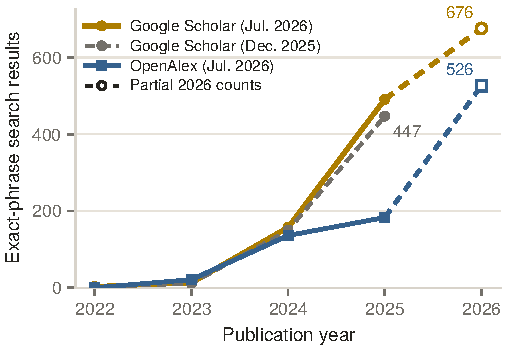
\includegraphics[width=\columnwidth]{../figures/fig_lrh_fulltext_mentions_space_optimized.pdf}
\caption{Exact-phrase search counts for \emph{linear representation hypothesis} in scholarly indexes have risen sharply since 2023.
This growing uptake motivates clarifying the different empirical claims associated with the shared label.
Appendix~\ref{sec:lrh-search} gives retrieval details.}
\label{fig:lrh-mentions}
\end{figure}

The LRH label’s widening use raises questions about each term in its name.
What does \emph{linear} refer to? A direction or subspace in activation space, or a linear map used to decode information from activations?
What counts as a \emph{representation}? Decodable information, structure that preserves relations in the represented domain, or something the model uses in computation?
Do these meanings define the same hypothesis, or do they imply distinct claims that can be tested separately?

\begin{figure*}[t]
\centering
% Figure 2: selected Tighter stack prism composition.
% Design and provenance: figures/data/claims/ and fig_claims.provenance.json.
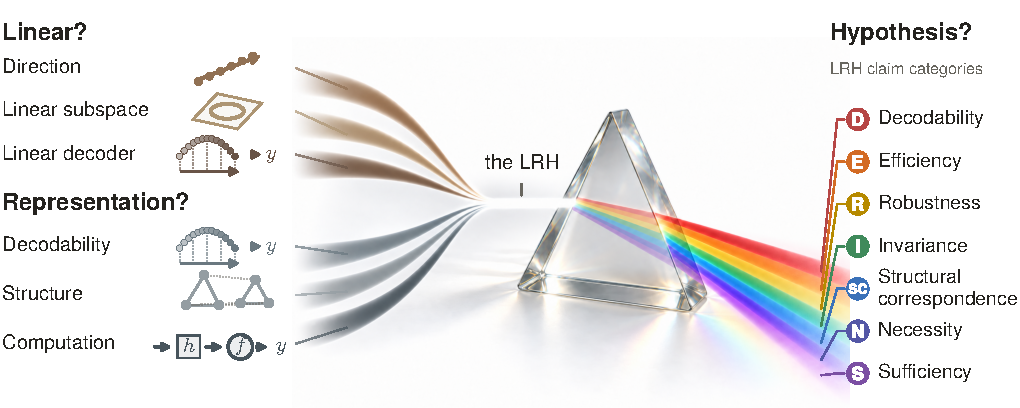
\includegraphics[width=\textwidth]{../figures/fig_claims_space_optimized.pdf}%

\caption{The \LRH{} label combines different meanings of linearity and representation into hypotheses with distinct empirical claims.
Linearity can refer to a direction, subspace, or decoder; linear decoding is compatible with activations on a nonlinear manifold.
Representation can mean decodability, relational structure, or use in model computation.
The seven claims on the right concern different properties and may co-occur.}
\label{fig:claims}
\end{figure*}

Prior work has developed several of these distinctions.
\citet{costa2025flat} discuss linear decodability, algebraic manipulation of model behavior, and decomposition into feature mixtures.
\citet{garg2026features} distinguish linear representation from \emph{linear accessibility}, the decodability criterion used here.
Finally, \citet{lee2026survey} formulate LRH claims for a model, representation location, feature, and evaluation distribution, and distinguish representation formation from use in computation.

Building on these distinctions, we develop a framework that organizes LRH claims into seven categories (Figure~\ref{fig:claims}) and defines assessment criteria for each.
We apply these criteria to compare evidence across studies, recording which claims are tested, what the results support, and under what experimental conditions.
For example, studies of truth directions in language models show strong decoding but mixed transfer, with necessity and mechanistic sufficiency untested (Table~\ref{tab:evidence-main}).
To illustrate these claims in a unified setting, we conduct experiments on number representations, finding gaps between accurate decoding, transfer across prompt variants, and behavioral control.
We first define the seven claims (Section~\ref{sec:weak-strong}), then examine evidence for observational claims (Section~\ref{sec:weak-lrh}) and causal claims (Section~\ref{sec:empirical-evidence}).

\begin{table*}[t]
\centering
\fontsize{8.2}{9}\selectfont
\setlength{\tabcolsep}{1.2pt}
\renewcommand{\arraystretch}{.98}
\begin{tabularx}{\textwidth}{@{}>{\centering\arraybackslash}m{7mm}>{\raggedright\arraybackslash}p{52mm}>{\raggedright\arraybackslash}X*{6}{>{\centering\arraybackslash}m{3.9mm}}*{2}{>{\centering\arraybackslash}m{4.5mm}}@{}}
\toprule
\multirow{2}{7mm}{\textbf{Type}} & \multirow{2}{52mm}{\textbf{Study and target}} & \multirow{2}{*}{\textbf{Candidate representation}} & \multicolumn{8}{c}{\textbf{Evidence by claim}} \\
\cmidrule(lr){4-11}
& & & \textbf{D} & \textbf{E} & \textbf{R} & \textbf{I} & \textbf{SC} & \textbf{N} & $\mathbf{S}_{\mathrm C}$ & $\mathbf{S}_{\mathrm M}$ \\
\midrule
\cellcolor{spectrumred!22}\textbf{D} & \citet{jobanputra2025subtract}: subtraction sign & Linear sign direction & \EvSupport{1} & \EvUntested & \EvUntested & \EvUntested & \EvUntested & \EvUntested & \EvUntested & \EvUntested \\
\cellcolor{spectrumred!22}\textbf{D} & \citet{kadlcik2025accurate}: number-token identity & Sinusoidal code; linear class scores & \EvSupport{3} & \EvUntested & \EvUntested & \EvUntested & \EvUntested & \EvUntested & \EvSupport{1} & \EvUntested \\
\cellcolor{spectrumorange!22}\textbf{E} & \citet{fu2026convergent}: modular residues & Fourier spectra; modular directions & \EvMixed{3} & \EvSupport{2} & \EvUntested & \EvUntested & \EvUntested & \EvUntested & \EvUntested & \EvUntested \\
\cellcolor{spectrumyellow!24}\textbf{R} & \citet{chanin2025absorption}: first-letter identity & Linear probes; SAE directions & \EvSupport{3} & \EvUntested & \EvAgainst{2} & \EvUntested & \EvUntested & \EvSupport{1} & \EvMixed{3} & \EvUntested \\
\cellcolor{spectrumgreen!22}\textbf{I} & \citet{gurnee2023language}: space and time & Space/time maps; selected neurons & \EvSupport{3} & \EvSupport{3} & \EvUntested & \EvSupport{2} & \EvUntested & \EvSupport{1} & \EvSupport{1} & \EvUntested \\
\cellcolor{spectrumgreen!22}\textbf{I} & \citet{marks2024geometry}: factual truth & Probe and mean-difference directions & \EvSupport{3} & \EvUntested & \EvUntested & \EvMixed{3} & \EvUntested & \EvUntested & \EvSupport{2} & \EvUntested \\
\cellcolor{spectrumgreen!22}\textbf{I} & \citet{bao2025probing}: factual truth & Linear truth-label probes & \EvSupport{3} & \EvSupport{2} & \EvUntested & \EvMixed{3} & \EvUntested & \EvUntested & \EvUntested & \EvUntested \\
\cellcolor{spectrumblue!22}\textbf{SC} & \citet{engels2025notall}: weekdays and months & Two-dimensional circular features & \EvUntested & \EvUntested & \EvSupport{1} & \EvSupport{1} & \EvSupport{3} & \EvUntested & \EvSupport{3} & \EvUntested \\
\cellcolor{spectrumblue!22}\textbf{SC} & \citet{hernandez2024linearity}: subject--object relations & Linear maps to object states & \EvMixed{3} & \EvUntested & \EvUntested & \EvSupport{2} & \EvMixed{3} & \EvUntested & \EvSupport{2} & \EvUntested \\
\cellcolor{spectrumblue!22}\textbf{SC} & \citet{park2025geometry}: categorical and hierarchical concepts & Final-layer directions and polytopes & \EvSupport{2} & \EvUntested & \EvSupport{1} & \EvUntested & \EvSupport{3} & \EvUntested & \EvSupport{1} & \EvUntested \\
\cellcolor{spectrumindigo!22}\textbf{N} & \citet{arditi2024refusal}: refusal & Selected mean-difference direction & \EvUntested & \EvUntested & \EvUntested & \EvUntested & \EvUntested & \EvSupport{3} & \EvSupport{3} & \EvSupport{1} \\
\cellcolor{spectrumindigo!22}\textbf{N} & \citet{tigges2023linear}: sentiment & Sentiment directions; traced circuits & \EvSupport{3} & \EvUntested & \EvSupport{3} & \EvMixed{2} & \EvUntested & \EvSupport{3} & \EvSupport{3} & \EvSupport{1} \\
\cellcolor{spectrumviolet!22}\textbf{S} & \citet{levy2025base10}: decimal digits & Circular digit codes & \EvSupport{3} & \EvUntested & \EvUntested & \EvSupport{1} & \EvSupport{2} & \EvUntested & \EvSupport{1} & \EvUntested \\
\cellcolor{spectrumviolet!22}\textbf{S} & \citet{nanda2023emergent}: player-relative state & Linear square--state directions & \EvSupport{3} & \EvUntested & \EvUntested & \EvUntested & \EvUntested & \EvUntested & \EvSupport{3} & \EvSupport{1} \\
\cellcolor{spectrumviolet!22}\textbf{S} & \citet{kantamneni2025trigonometry}: integer arithmetic & Linear and periodic helix & \EvUntested & \EvUntested & \EvUntested & \EvSupport{1} & \EvSupport{3} & \EvSupport{2} & \EvSupport{3} & \EvSupport{2} \\
\cellcolor{spectrumviolet!22}\textbf{S} & \citet{makelov2023subspace}: factual recall and IOI & MLP and residual-stream directions & \EvUntested & \EvUntested & \EvSupport{2} & \EvUntested & \EvUntested & \EvSupport{1} & \EvSupport{3} & \EvMixed{3} \\
\cellcolor{spectrumviolet!22}\textbf{S} & \citet{zhou2024fourier}: integer addition & Low/high-frequency Fourier components & \EvUntested & \EvUntested & \EvUntested & \EvUntested & \EvSupport{3} & \EvSupport{3} & \EvUntested & \EvSupport{2} \\
\bottomrule
\end{tabularx}
\caption{Evidence for the seven \LRH{} claims, with causal ($S_{\mathrm C}$) and mechanistic ($S_{\mathrm M}$) sufficiency rated separately.
Rows are grouped by the claim category used for this comparison.
D, E, R, I, SC, and N denote decodability, efficiency, robustness, invariance, structural correspondence, and necessity.
IOI denotes indirect-object identification.
Claim colors follow Figure~\ref{fig:claims}.
Green, amber, crossed red, and empty markers indicate support, mixed evidence, counterevidence, and no reported test.
Fill levels indicate limited, moderate, or strong evidence.
The excerpt covers 17 of 30 studies, see full coverage in Appendix Table~\ref{tab:evidence-full}).}
\label{tab:evidence-main}
\end{table*}

\begin{figure*}[t]
\centering
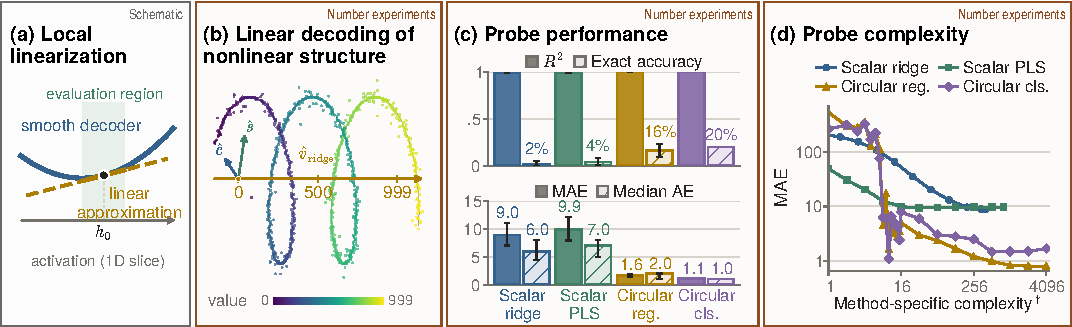
\includegraphics[width=\textwidth]{../figures/fig_decodability_efficiency_space_optimized.pdf}
\caption{Accurate probing is compatible with nonlinear activation structure.
(a) A smooth nonlinear decoder is approximately linear within a small evaluation region, allowing a linear probe to predict the target there.
(b) Ridge predictions and a sine--cosine pair from circular regression for 1,000 values (800 used for fitting).
The gray helix traces the target code.
(c) Probes on 100 test-value centroids of Llama-3.1-8B layer-10 addition-formula activations, averaged over 20 contexts.
Whiskers give 95\% test-value bootstrap intervals for fixed fits, except for the classifier, whose results are available only as aggregates.
(d) Test MAE versus complexity on the same activations and fixed value-disjoint split (log axes).
$\dagger$~Complexity denotes ridge effective degrees of freedom, PLS component count, or circular-code dimension.
See Appendix Figure~\ref{fig:circular-components} for all ten circular components and Appendices~\ref{sec:numerical-probe-setup} and \ref{sec:geometric-illustrations} for setup and constructions.}
\label{fig:decodability}
\end{figure*}

% Figure 4: robustness, invariance, and structural correspondence.
\begin{figure*}[t]
\centering
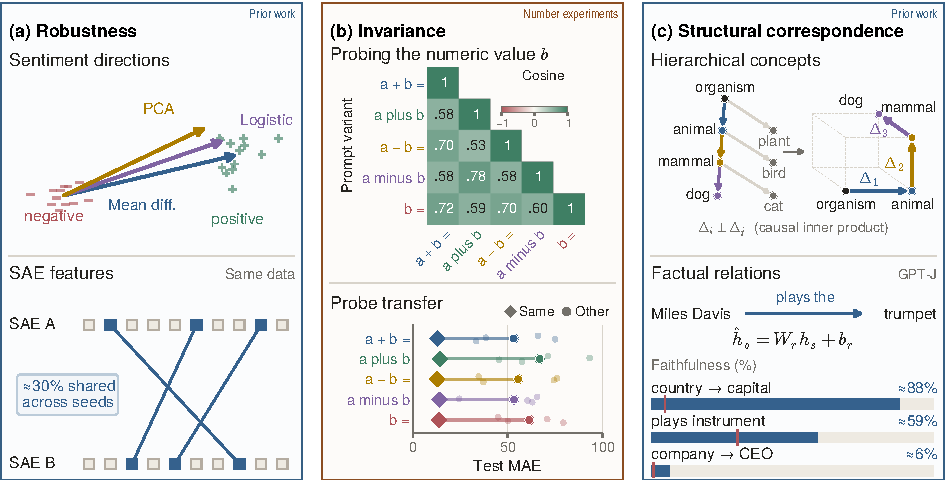
\includegraphics[width=\textwidth]{../figures/fig_robustness_invariance_structure_space_optimized.pdf}
\caption{Robustness and invariance receive mixed support, with structural correspondence observed for specific semantic relations.
The panels show agreement across estimates, transfer across prompts, and semantic relations in activation space.
(a) Sentiment directions agree across methods \citep{tigges2023linear} (top), but about 30\% of SAE features are shared across seeds \citep{paulo2026sparse} (bottom).
(b) Numerical probe directions vary across prompt variants (top), and transferred probes have large errors (bottom).
Small circles show transfer errors for individual target variants; large circles show their mean, and diamonds show within-variant error.
Summaries average six models and eleven relative layers on one fixed value-disjoint split.
(c) Orthogonal differences can encode a concept hierarchy \citep{park2025geometry} (top).
For factual relations, relation-specific linear maps predict object states $\hat h_o$ from subject states $h_s$, with varying faithfulness across relations \citep{hernandez2024linearity} (bottom).
Bars measure this faithfulness by first-token agreement with the full model; red marks show random guess.}
\label{fig:robustness-invariance-structure}
\end{figure*}


% Figure 5: literature evidence and numerical-subspace deletion.
\begin{figure*}[t]
\centering
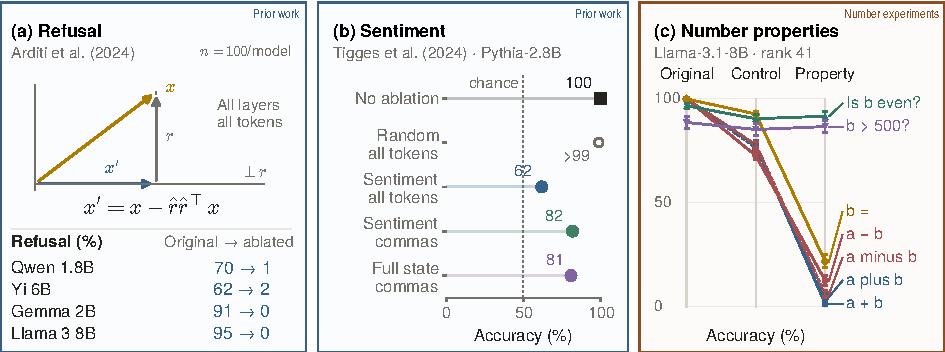
\includegraphics[width=\textwidth]{../figures/fig_causal_use_space_optimized.pdf}
\caption{Direction ablation and subspace deletion test causal necessity through changes in behavior.
(a) Removing an activation's component along the refusal direction suppresses refusal on harmful instructions in four models \citep{arditi2024refusal}.
(b) Ablating a sentiment direction lowers accuracy on originally correct SST examples containing commas \citep{tigges2023linear}.
(c) Deleting the subspace fitted to number properties impairs arithmetic and copying more than parity and comparison.
\emph{Property} and \emph{Control} delete rank-41 spans fitted on addition formulas with true or shuffled property labels.
The contrast with \emph{Control} supports a behavioral role for the property subspace.
Whiskers in (c) give 95\% source-value-cluster bootstrap intervals, conditional on ten fitted bases.}
\label{fig:causal-use}
\end{figure*}


% Queue the property-decoding and steering figures on consecutive page tops.
\begin{figure*}[t]
\centering
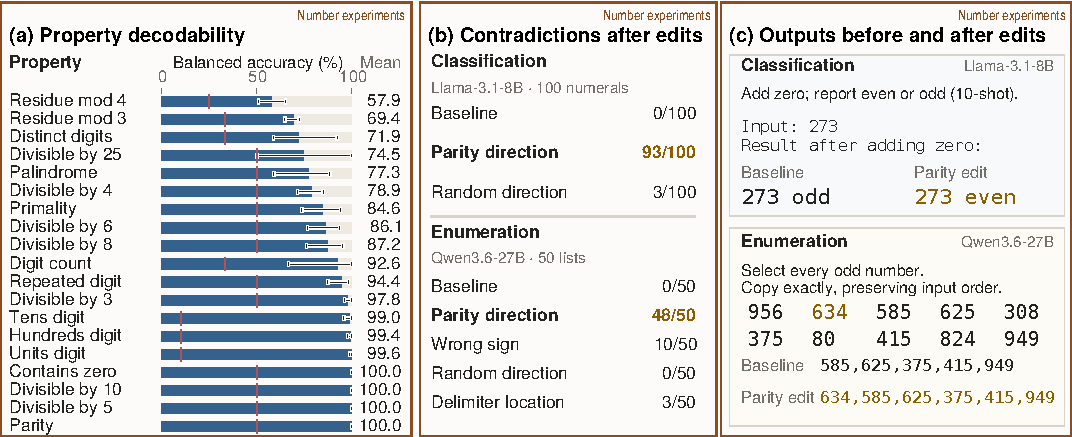
\includegraphics[width=\textwidth]{../figures/fig_number_property_evidence_main_space_optimized.pdf}
\caption{Probes decode number properties, and parity-direction edits can change classification labels or membership in a list.
(a) Mean balanced accuracy of probes on full Llama-3.1-8B activations.
Whiskers show ranges across six to ten value-disjoint splits, each testing every class.
Red ticks mark chance.
(b) Contradictions after parity edits and controls on 100 classification queries and 50 enumeration lists, all correct before editing.
(c) In classification, the edit flips the parity label while preserving the numeral; in enumeration, it adds an even numeral to an otherwise unchanged list of odd numerals.
Both outputs conflict with the numeral's parity or the request for odd numbers.
Edits add separately fitted directions to activations, with doses chosen on development data (Appendix~\ref{sec:numerical-control-dimension}).}
\label{fig:number-property-accessibility-main}
\end{figure*}

\begin{figure*}[t]
\centering
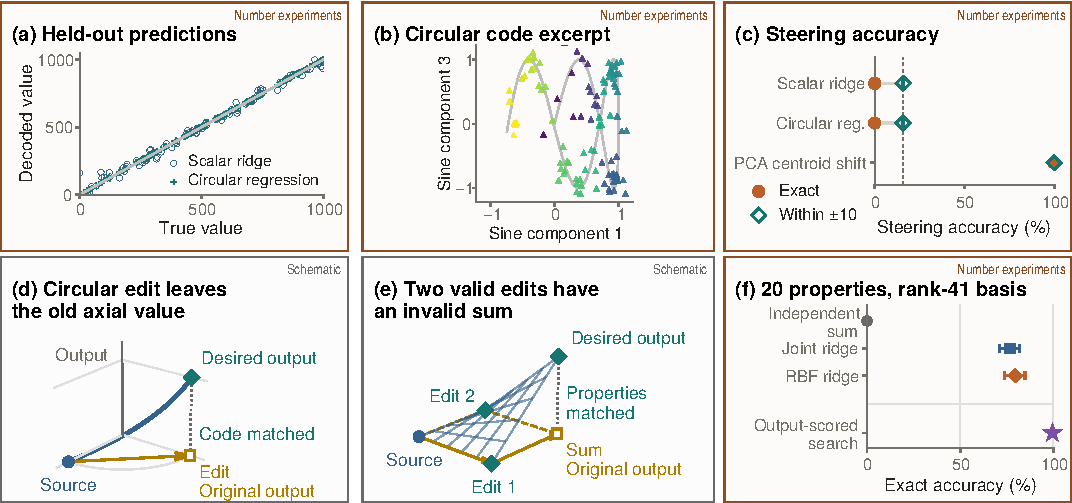
\includegraphics[width=\textwidth]{../figures/fig_numerical_sufficiency_atlas_space_optimized.pdf}
\caption{Probe-derived edits yield little control despite accurate numerical decoding.
(a,b) Scalar ridge and circular regression decode values and codes from 100 individual Llama-3.1-8B development prompts.
(c) On these prompts, edits from the same fits yield no exact target outputs (2,000 per method); a PCA centroid shift succeeds.
The dotted line gives no-edit accuracy within $\pm10$.
(d,e) Matching a circular code or summing valid property edits can preserve the source output.
(f) Joint predictors use source activations and patch displacements, with different doses from the independent sum (400 edits, 20 source prompts).
Output-scored search evaluates all 100 source prompts (2,000 edits).
Whiskers in (c,f) give 95\% source-prompt bootstrap intervals for fixed fits (Appendices~\ref{sec:numerical-probe-setup} and~\ref{sec:numerical-control-dimension}).}
\label{fig:numerical-sufficiency-atlas}
\end{figure*}



\section{A Spectrum of \LRH{} Claims}
\label{sec:weak-strong}

We distinguish seven kinds of claim about decodability, activation-space structure, and model computation (Figure~\ref{fig:claims}).
Each concerns a different property, and several can hold for the same representation.
This section describes the claims informally; Appendix~\ref{sec:claim-formalization} gives formal definitions.

\emph{Decodability} is tested by fitting a linear probe to labeled activations and evaluating its target predictions on held-out examples.
This criterion underlies linear-probe analyses in computer vision and natural language processing \citep{alain2018understanding,liu2019linguistic,belinkov2022probing}.
\emph{Efficiency} adds a cost criterion, comparing probe complexity at comparable predictive performance \citep{gurnee2023language}, or complexity and fit jointly through measures such as description length \citep{voita2020information}.

Three further claims concern structures identified in model activations.
\emph{Robustness} requires directions or subspaces to agree across repetitions that vary the sampled examples, analysis choices, or model-training settings.
For example, sentiment directions and sparse-autoencoder features are favorable and unfavorable cases under this criterion \citep{tigges2023linear,chanin2025absorption}.
\emph{Invariance} requires a probe or the direction or subspace it identifies to transfer across target-preserving input variations, domains, or value ranges.
A test may assess frozen-probe accuracy, agreement between directions or subspaces identified separately in each setting, or both \citep{gurnee2023language,marks2024geometry,park2024linear}.
\emph{Structural correspondence} requires activation-space objects assigned to target values to preserve specified target relations, such as distances or operations \citep{shepard1970secondorder,kriegeskorte2008representational,shea2018structural}.
Representative findings are word vector algebra, circular representations, and categorical or hierarchical geometry \citep{mikolov2013linguistic,engels2025notall,park2025geometry}.

These first five categories concern observational claims about decodability and activation-space structure; the final two concern causal claims about model computation.
\emph{Necessity} requires that selectively removing information about the target property lowers performance on a relevant task \citep[Sec.~3.2]{harding2023operationalising}.
We assess causal and mechanistic \emph{sufficiency} separately.
\emph{Causal sufficiency} tests whether editing activations to represent a target value produces the predicted behavior \citep{heimersheim2024patching}.
\emph{Mechanistic sufficiency} further requires the hypothesized representation and transformations to explain ordinary computation and predict intervention effects, as in analyses of arithmetic \citep{zhou2024fourier,kantamneni2025trigonometry,feucht2026arithmetic}.
The connection to ``ordinary'' computation matters because interventions may result in computation that is ``unnatural'' for the model, e.g., by recruiting dormant pathways \citep{makelov2023subspace}.

Necessity and causal sufficiency provide complementary tests: redundant pathways can make information sufficient without making it necessary, and interacting components can make it necessary without making it sufficient \citep{heimersheim2024patching}.
The following sections examine what prior work and illustrative experiments establish for each LRH claim.

\section{Evidence for Observational Claims}
\label{sec:weak-lrh}

We now examine how prior work tests the five observational claims (Table~\ref{tab:evidence-main}) and conduct experiments with number representations, focusing on decoding performance, transfer across prompt variants, and activation-space structure.

\subsection{Decodability}
\label{sec:decodability}

Linear decodability has the broadest evidence base in our review (Table~\ref{tab:evidence-main}, column D).
Linear probes predict geographic locations and dates from activations elicited by place names and event descriptions \citep{gurnee2023language}, distinguish representations of true and false statements \citep{marks2024geometry}, and decode board states from a model trained to predict Othello moves \citep{nanda2023emergent}.

However, accurate linear decoding is compatible with nonlinear activation-space structure.
A linear probe can locally approximate a smooth nonlinear decoder (Figure~\ref{fig:decodability}a).
For number representations, \citet{kantamneni2025trigonometry} fit a generalized helix whose linear magnitude component permits scalar decoding.
By accounting for nonlinear helical structure, \citet{kadlcik2025accurate} improve exact-match accuracy with a circular classifier based on Fourier features.

\begingroup
\clubpenalty=10000
\textbf{Number experiments.} We compare these scalar and circular approaches as tests of the decodability claim, fitting two probes of each kind to the same Llama-3.1-8B activations.
Scalar probes predict numerical values directly, using ridge regression or partial least squares (PLS) \citep{wold2001pls,heinzerling2024monotonic}; circular probes use sine--cosine encodings of those values.
We average activations across addition prompts for each number and evaluate the probes on unseen values (Appendix~\ref{sec:numerical-probe-setup}).
All four attain $R^2>.99$, yet mean absolute error (MAE) is 1.1--1.6 for circular probes and 9.0--9.9 for scalar probes (Figure~\ref{fig:decodability}c).
Combining a scalar prediction with a predicted sine--cosine pair traces an approximate helix in the probe outputs (Figure~\ref{fig:decodability}b).
A plausible interpretation of these results is that scalar probes recover a linear magnitude component, while other activation components vary nonlinearly with numerical value.
More generally, this exemplifies how linear decodability places few constraints on the full representational geometry.
As we will see  (Section~\ref{sec:sufficiency}) this geometric ambiguity leads to a decodability-control gap: interventions based on probe predictions can leave behaviorally relevant components unchanged.
\par
\endgroup

\subsection{Efficiency}

The efficiency claim concerns the complexity needed to attain a given decoding accuracy.
Evidence for this claim includes linear probes that perform similarly to larger multilayer perceptrons when predicting locations and dates \citep{gurnee2023language} or survey response distributions for demographic groups \citep{jahanparast2026opinions}.
Minimum-description-length probing measures this trade-off in bits by combining the costs of describing the probe and encoding the labels with it \citep{voita2020information}.

\textbf{Number experiments.} We examine this accuracy--complexity trade-off by varying regularization or dimensionality for the probes from Section~\ref{sec:decodability}, using the same activations and value split (Figure~\ref{fig:decodability}d; six-model sweep in Appendix Figure~\ref{fig:probe-capacity-paths}).
At the smallest tested settings, scalar probes have lower error than circular probes.
With ten-dimensional codes, however, the circular probes become substantially more accurate.
One plausible explanation is that scalar probes recover the generalized helix's linear magnitude component at low complexity, while circular probes gain precision by capturing additional periodic structure once their codes have enough components.
On this interpretation, the efficiency comparison---and, more broadly, whether number representations count as ``linear''---depends on whether the aim is to recover approximate magnitude or make finer distinctions.

\subsection{Robustness}

Tests of robustness ask whether repeated analyses identify similar directions or subspaces.
For sentiment, \citet{tigges2023linear} find similar directions using mean differences, logistic regression, and principal component analysis (Figure~\ref{fig:robustness-invariance-structure}a, top).

However, \citet{paulo2026sparse} find that individual SAE features vary even when only the initialization seed changes.
Across runs trained on identical data, only about 30\% of features have matching encoder and decoder directions (Figure~\ref{fig:robustness-invariance-structure}a, bottom).
The features associated with a concept also change with SAE width and sparsity \citep{chanin2025absorption}.
Individually variable features can nevertheless concentrate in reproducible subspaces \citep{gerasimov2026unstable}.
A robustness claim should therefore specify whether it concerns individual directions or a shared subspace.

\subsection{Invariance}

The invariance claim concerns whether a probe or activation-space structure transfers across contexts in which the same target property is expressed.
For truth probes, \citet{bao2025probing} find uneven transfer from factual statements to question-answering tasks, with accuracy and calibration varying across conditions.
Probes trained on affirmative statements can also fail on negated statements, depending on the model and topic \citep{bao2025probing}.

\textbf{Number experiments.} We test this invariance claim for numerical magnitude by keeping numerical values fixed across five prompt variants.
For each variant, we average activations over contexts for each number and fit a PLS magnitude probe.
We compare the fitted directions and test each probe unchanged on the other variants.
Averaged over six models and eleven relative layers, the directions agree only moderately (Figure~\ref{fig:robustness-invariance-structure}b, top), and transfer roughly quadruples decoding error relative to evaluation within the training variant (Figure~\ref{fig:robustness-invariance-structure}b, bottom).
Aligning mean activations across variants using training data reduces this error, but a substantial gap persists (Appendix Figure~\ref{fig:prompt-family-pls-transfer}).
The transfer gap shows that decodability within a prompt variant does not by itself establish invariance across variants.

\subsection{Structural Correspondence}

Structural correspondence is tested by checking whether activation-space geometry or transformations preserve target relations.
For hierarchical concepts, \citet{park2025geometry} find that successive refinements such as animal\,$\to$\,mammal\,$\to$\,dog correspond to approximately orthogonal vector differences (Figure~\ref{fig:robustness-invariance-structure}c, top).
\citet{hernandez2024linearity} fit relation-specific linear maps from subject representations to states predicting related objects, such as a musician's instrument (Figure~\ref{fig:robustness-invariance-structure}c, bottom).

However, \citet{hernandez2024linearity} find that these maps perform poorly for some relations even when the model predicts correctly.
Success of interventions using linear maps correlates positively with subject--object co-occurrence frequency in pretraining data \citep{merullo2025linear}, suggesting that exposure may partly explain this variation.
The evidence supports structural correspondence for particular semantic relations and activation-space structures.

\section{Evidence for Causal Claims}
\label{sec:empirical-evidence}

The previous section examined decodability and activation-space structure; we now turn to necessity and causal sufficiency.

\subsection{Necessity}
\label{sec:necessity}

Necessity tests ask whether removing about the target property disrupts the behavior it is thought to support \citep[Sec.~3.2]{harding2023operationalising}.\footnote{
Removal generally changes the distribution of activations, potentially producing off-distribution states \citep[Appendix~A]{mcgrath2023hydra}.
Behavioral changes can therefore reflect distribution shift as well as loss of target information.}
Removal methods include projecting out a probe direction and erasing linearly decodable concept information \citep{ravfogel2020null,belrose2023leace}.
For example, \citet{arditi2024refusal} suppress refusal on harmful instructions by ablating a refusal direction (Figure~\ref{fig:causal-use}a).
Jointly removing additional refusal directions can suppress refusal further \citep{wollschlager2025geometry}.
Ablating a sentiment direction also lowers classification accuracy \citep{tigges2023linear} (Figure~\ref{fig:causal-use}b).

\textbf{Number experiments.} We test this necessity claim by deleting a subspace of number-token activations in Llama-3.1-8B.
The subspace is fitted on addition formulas to magnitude and nineteen categorical properties (Figure~\ref{fig:number-property-accessibility-main}a).
Because deletion can remove other task-relevant information, we also delete a rank-matched subspace fitted to shuffled labels.
Deleting the property subspace sharply reduces arithmetic and copying accuracy, with smaller effects on parity and comparison (Figure~\ref{fig:causal-use}c).
The shuffled-label control is less disruptive on arithmetic and copying, supporting a task-dependent behavioral role for the fitted subspace as a whole.

\subsection{Sufficiency}
\label{sec:sufficiency}

Causal sufficiency tests ask whether whether editing activations to represent a target value produces the predicted behavior.
Interventions can correct a proposed misrepresentation \citep[Sec.~3.3]{harding2023operationalising} or steer activations toward a desired outcome \citep{li2023iti,tigges2023linear,zou2023representation}.
For example, Steering activations along a refusal direction induces refusal on harmless instructions \citep{arditi2024refusal}.
However, decoding accuracy alone does not ensure control: truth probes with similar accuracy yield different steering effects \citep{marks2024geometry}.
For numbers, repairing embeddings using sinusoidal structure improves arithmetic \citep{kadlcik2025accurate}, yet edits from accurate circular digit probes produce the intended number in only 10--15\% of copying trials \citep{levy2025base10}.

\textbf{Number experiments.} We test whether probe-derived edits can control addition: editing the represented 0 in \texttt{92+0=} to 1 should produce 93.
We fit scalar ridge and circular-regression probes on individual prompts and use the same fits and source prompts for decoding and steering.
The probe pseudoinverse maps target--source differences in scalar values or sinusoidal codes into activation edits (Appendix~\ref{sec:numerical-probe-geometry}).
These edits produce no exact target outputs, but adding differences between target and source activation centroids \citep{wurgaft2026manifold} or patching activations from matched target prompts exceeds 99\% exact accuracy at the same site (Figure~\ref{fig:numerical-sufficiency-atlas}a--c).
The probe-derived edits preserve activation components that do not affect probe predictions; downstream use of these components could explain the control gap.

Because the successful edits change multiple components, we test sufficiency more selectively with parity.
A direction fitted on Llama-3.1-8B parity questions flips labels while preserving numerals in 93 of 100 cases, versus 3 for a norm-matched random direction (Figure~\ref{fig:number-property-accessibility-main}b,c).
Directions fitted on addition formulas yield no such contradictions on parity questions despite perfect in-format decoding, indicating context-dependent control.
A Qwen3.6-27B direction also inserts an even numeral into a list of odd numerals, although reversing the direction or editing a delimiter can also induce contradictions, limiting specificity (Appendix~\ref{sec:property-reasoning}).

We also test whether property-based edits combine to control arithmetic within the subspace used for deletion.
The independent method predicts and sums edits from each property's source and target labels.
Joint predictors additionally use source activations projected into the subspace to predict coefficients of activation differences between source and matched target prompts (Appendix~\ref{sec:property-coefficient-control}).
On held-out source prompts, the independent sum yields no exact target outputs, versus 77\% exact accuracy for joint ridge and 80\% for the radial-basis-function predictor (Figure~\ref{fig:numerical-sufficiency-atlas}f).
The methods differ in inputs, training targets, and doses, and evaluation reuses target values from training.
A separate search selecting edits by the requested output reaches 99.5\% accuracy in the same subspace (Appendix~\ref{sec:property-coefficient-control}).
Causal sufficiency here depends on the information and procedure used to construct and select edits.

\section{Discussion and Conclusions}

The reviewed evidence supports linear decodability across many settings, with more variable findings for geometry, transfer, and behavioral control.
The number experiments make these differences concrete: magnitude is accurately decodable, yet probe transfer and behavioral control depend on context and intervention construction.

Scalar and circular probes both use linear maps from activations but predict different target encodings.
Although both attain high $R^2$, circular probes ultimately yield lower numerical error, reversing the ordering seen at low complexity (Figure~\ref{fig:decodability}c,d).
This pattern is consistent with scalar probes recovering linear magnitude and circular probes capturing additional periodic structure.
On this interpretation, accurate linear decoding coexists with nonlinear structure that contributes to finer numerical distinctions.

For magnitude, the decoding relationship also changes with prompt context.
Transfer gaps after mean alignment suggest that this dependence extends beyond a shift in average activations (Appendix Figure~\ref{fig:prompt-family-pls-transfer}).
The parity-steering results extend this context dependence to interventions.
A direction fitted on parity questions changes labels while preserving numerals (Figure~\ref{fig:number-property-accessibility-main}b), yet directions fitted on addition produce no such contradictions despite perfect in-format decoding.

Control also varies with edit construction within a fixed subspace.
Deleting the property subspace disrupts arithmetic and copying more than a shuffled-label control, yet summing independent property edits gives no exact target outputs (Figures~\ref{fig:causal-use}c and~\ref{fig:numerical-sufficiency-atlas}f).
Joint predictors and output-scored search nevertheless achieve substantial control within that same subspace.
These procedures differ in inputs, training targets, and doses, with search additionally using behavioral feedback.
The same subspace can therefore be behaviorally consequential under deletion while supporting sharply different control outcomes across edit procedures.

These successful edits establish causal sufficiency under the tested intervention conditions.
Mechanistic sufficiency further entails explaining how ordinary computation produces and transforms the relevant activation states, and predicting intervention effects on that computation.
Overall, the seven claims distinguish these coexisting properties, giving a more informative account of representations than a single verdict that they are ``linear''.

\section*{Limitations}

The review prioritizes cited studies with accessible full text and adds cases to cover the seven claim categories (Appendix~\ref{sec:evidence-comparison}).
This purposive selection leaves the prevalence of claims and evidential gaps in the wider literature unmeasured.
The evidence ratings also involve judgments about how directly each test bears on a claim.
LLMs drafted ratings and summaries, which were checked against source papers and adjudicated with AI assistance; agreement among independent human coders was not measured.

Our experiments illustrate relationships among the claims for numerical properties in selected models and tasks.
How the transfer and control patterns generalize to other concepts is untested.
The helical interpretation is based on selected probe outputs, which leave the full activation-space geometry undetermined.
The control results apply to the tested probe fits, activation site, and edit rules.

Independent and joint predictors differ in inputs, training targets, and doses, so their comparison does not isolate an advantage from joint prediction.
The joint predictors are evaluated on new source prompts but reuse target values from training.
The separate search uses the requested output to select edits; without matched searches in random, principal-component, or shuffled-label subspaces, its success leaves the property subspace's specific contribution unresolved.

The bootstrap intervals reflect variation in evaluation examples with the probes or bases held fixed, so they exclude uncertainty across refits.
The prompt-transfer results additionally use a single value partition, leaving sensitivity to the split untested.

\bibliography{refs}

\clearpage
\appendix
\raggedbottom
\appendixcontents

\renewcommand{\dbltopfraction}{.95}
\renewcommand{\textfraction}{.02}

\appendixsection{Search Procedure for Figure~\ref{fig:lrh-mentions}}
\label{sec:lrh-search}

Figure~\ref{fig:lrh-mentions} counts scholarly database results for the exact phrase \emph{``linear representation hypothesis''}, once per result.
The gray \href{https://scholar.google.com/}{Google Scholar} series was collected in December 2025 \citep{lee2026survey}; the ochre Google Scholar and blue \href{https://openalex.org/}{OpenAlex} series were collected on 31 July 2026.
Google Scholar reports approximate totals under default settings, potentially including multiple versions and references; OpenAlex \texttt{search.exact} searches titles, abstracts, and indexed full text, including references.
Because these retrieval procedures differ, the series should be interpreted separately.
Dashed segments indicate partial 2026 counts.

As a manual check of retrieved mentions, we examined passages from the 206-document full-text corpus described in Appendix~\ref{sec:evidence-comparison}.
This corpus comprises accessible PDFs from candidates with at least one citation and detected main-body phrase matches.
We extracted each phrase occurrence with the preceding and following paragraphs and merged overlapping context windows into \emph{episodes}.

One author reviewed 60 episodes from 54 documents in two 30-episode samples, each containing ten episodes selected at random from each of three citation-rank groups.
The review was completed on 3 October 2026 using an interface that hid machine judgments and sampling groups.
Of these episodes, 47 (78\%) were classified as substantive uses of the LRH, including explanations of the hypothesis, methodological motivation, and discussion of favorable or contrary evidence.
The remaining episodes were twelve bibliography entries and one structural fragment.
This author audit involved no recruited participants or crowdworkers and collected no participant data.
The \href{https://github.com/bheinzerling/linear-representation-hypothesis/tree/main/data/literature/human_audit}{released audit records} contain the case-level status and purpose judgments, episode identifiers, and sampling phases, with a script that reproduces the counts and comparisons with the machine annotations.

We classified all 376 episodes using two \texttt{gpt-5.6-sol} coding agents with high reasoning effort, assigning one primary annotation per episode.
Under this scheme, an episode is substantive when it articulates an LRH proposition, adopts it as a premise, or evaluates it.
Applying the scheme identifies at least one substantive episode in 182 of 203 distinct papers (90\%) after merging three verified version pairs.
As a consistency check, the agents double-coded 60 episodes and agreed on all episode statuses, although agreement can reflect shared model errors.
On those same episodes, each agent agreed with the author's status judgment in 58 of 60 cases.
Table~\ref{tab:lrh-substantive-annotations} summarizes the author audit and the automated classifications of the audit sample and full corpus.
These results indicate frequent substantive engagement within the selected corpus.
Estimating its prevalence among the database results in Figure~\ref{fig:lrh-mentions} requires representative sampling.

\begin{table}[H]
\centering
\small
\setlength{\tabcolsep}{3pt}
\begin{tabular}{@{}lrrrr@{}}
\toprule
Annotation & $n$ & Substantive & Non-subst. & Unclear \\
\midrule
Human & 60 & 47 (78\%) & 13 & 0 \\
LLM (audit) & 60 & 47 (78\%) & 12 & 1 \\
LLM (corpus) & 376 & 314 (84\%) & 56 & 6 \\
\bottomrule
\end{tabular}
\caption{Episode-status counts for the author audit, the same episodes coded by both LLM agents, and the full LLM-coded corpus.
The LLM audit counts are identical for both agents.
Non-substantive episodes are bibliography entries or structural fragments; unclear cases have insufficient context.}
\label{tab:lrh-substantive-annotations}
\end{table}

\clearpage
\onecolumn
\appendixsection{Formal Claim Definitions}
\label{sec:claim-formalization}

Table~\ref{tab:claim-criteria} formalizes the seven claim categories in Section~\ref{sec:weak-strong}.
For target $C(x)$ and activation $h(x)$ at a layer and position, a linear probe $a$ has held-out error $L(a)=\E[e(a(h(x)),C(x))]$ with task-appropriate error $e$.
This error is evaluated on inputs independent of fitting data, with a fixed decoding rule for categorical scores.
In the criteria below, $\epsilon$ bounds error or discrepancy, and $\approx$ denotes approximate agreement.

Harding's information criterion corresponds to decodability \citep[Sec.~3.1]{harding2023operationalising}, selective removal tests the use criterion and necessity \citep[Sec.~3.2]{harding2023operationalising}, and correcting misrepresentation provides partial evidence for causal sufficiency \citep[Sec.~3.3]{harding2023operationalising}.
These representation criteria apply to linear and nonlinear candidates.

\begin{table}[H]
\centering
\small
\setlength{\tabcolsep}{5pt}
\renewcommand{\arraystretch}{1.08}
\begin{tabularx}{\textwidth}{@{}>{\raggedright\arraybackslash}p{24mm}>{\raggedright\arraybackslash}p{55mm}>{\raggedright\arraybackslash}X@{}}
\toprule
\textbf{Claim} & \textbf{Informal statement} & \textbf{Formal criterion and test conditions} \\
\midrule
Decodability & A linear probe fitted to labeled activations predicts a target on held-out examples from the evaluation distribution.
& $\displaystyle L(a)\leq\epsilon$. \\
\addlinespace[5pt]
Efficiency & A linear probe has lower complexity or uses fewer labels at comparable predictive performance, or has a shorter total description length.
& For comparator $b$ on the same evaluation distribution and cost measure $K$, require
\par $\displaystyle L(a)\leq L(b)+\delta,\qquad K(a)<K(b)$.
\par The tolerance $\delta\geq0$ permits an error increase; $K$ measures complexity or labels used for fitting.
The description-length version requires $K(a)<K(b)$ with $K$ combining complexity and fit. \\
\addlinespace[5pt]
Robustness & Directions or subspaces agree across repetitions that vary the sampled examples, analysis choices, or model-training settings.
& $\displaystyle U\approx V$ for directions or subspaces $U,V$ obtained across the tested repetitions.
The claim specifies which samples, analysis choices, or training settings may vary. \\
\addlinespace[5pt]
Invariance & A probe or the direction or subspace it identifies transfers across target-preserving input variations, domains, or value ranges.
& After a change that preserves target semantics, require
\par $\displaystyle L(a)\leq\epsilon\qquad\text{and/or}\qquad U\approx V$.
\par The probe $a$ is fitted in the original setting and frozen during evaluation on the new distribution; $U,V$ are fitted separately in the two settings.
The claim selects probe transfer, agreement between structures, or both. \\
\addlinespace[5pt]
Structural correspondence & Activation-space objects assigned to target values preserve specified target relations, such as distances or operations.
& Let $\phi$ assign activation-space objects to target values.
For the evaluated values $u,v$ or tuples $\mathbf c$, compare the target and activation-space relations:
\par $\displaystyle \begin{gathered}d\!\left(\phi(u),\phi(v)\right)\approx\rho(u,v),\\ g\!\left(\phi(\mathbf c)\right)\approx\phi\!\left(f(\mathbf c)\right).\end{gathered}$
\par The target space uses distance $\rho$ and operation $f$; the activation space uses $d$ and $g$.
The map $\phi$ acts componentwise on tuples. \\
\addlinespace[5pt]
Necessity & Selectively removing candidate information prevents the specified behavior at the required fidelity.
& For expected behavioral error $L_B$ under background conditions $B$, selective removal $I_-$, and unedited baseline $I_0$, require
\par $\displaystyle L_B(I_0)\leq\epsilon<L_B(I_-)$.
\par Removal reduces candidate information and preserves other relevant information; inputs, the error metric, and $\epsilon$ are fixed. \\
\addlinespace[5pt]
Sufficiency & Causal sufficiency: candidate content produces predicted behavior.
Mechanistic sufficiency: the representation and transformations explain ordinary computation and intervention effects.
& \emph{Causal:} $L_B^*(I_c)\leq\epsilon<L_B^*(I_0)$, where $I_c$ sets candidate content to $c$ and $L_B^*$ measures expected error relative to the predicted target behavior.
The comparison fixes background $B$, other relevant information, and the intervention procedure.
\par \emph{Mechanistic:} for computation $F_I$ and the hypothesized mechanism $\widehat F_I$,
\par $\displaystyle \E_{x,I}\!\left[\Delta\!\left(\widehat F_I(x),F_I(x)\right)\right]\leq\epsilon$.
\par $I$ ranges over the identity and specified content interventions; $\Delta$ compares internal computation and output behavior. \\
\bottomrule
\end{tabularx}
\caption{Informal statements and formal criteria for the seven claim categories.
For efficiency, invariance, and structural correspondence, a concrete claim specifies which comparison or relation it tests.}
\label{tab:claim-criteria}
\end{table}

\clearpage
\twocolumn

\appendixsection{Expanded Evidence Comparison}
\label{sec:evidence-comparison}

Table~\ref{tab:evidence-full} compares 11 citation-prioritized studies from the OpenAlex exact-phrase search in Figure~\ref{fig:lrh-mentions} with 19 studies drawn from the broader literature review.
For the exact-phrase corpus, 519 of 567 OpenAlex candidates resolved to Semantic Scholar \citep{ammar2018semantic}.
Among these matches, we sought full text for the 311 candidates with at least one citation, in citation order, retaining 206 documents with main-body phrase matches.
To complement this citation-prioritized selection, the broader review includes favorable and contrary findings across every claim category.
Both tables group studies by the claim category used to organize the comparison.
Table~\ref{tab:evidence-main} extracts cases covering each category from the full comparison.

The rubric evaluates each claim category on its own.
For decodability and efficiency, the criteria concern held-out prediction and efficiency relative to a comparator.
From robustness through structural correspondence, they concern reproducibility of directions or subspaces, transfer between contexts or values, and preservation of target relations.
Necessity concerns selective removal and the resulting loss of behavioral fidelity.
Sufficiency is rated separately for interventions that produce predicted behavior ($S_{\mathrm C}$) and for explanations of ordinary computation and intervention effects ($S_{\mathrm M}$).
The causal ratings refer to the reported activation sites, backgrounds, intervention procedures, and behavioral metrics.

Each rating records the strength and direction of the evidence for its claim category.
For strength, limited denotes a narrow or indirect analysis, moderate denotes a direct test under restricted conditions, and strong denotes multiple direct tests within a study.
For direction, mixed denotes materially different, condition-dependent outcomes, and counterevidence denotes a conflict with the candidate claim.
In these ratings, partial effects can support a criterion without establishing it at every fidelity threshold.
The table abbreviates sparse autoencoder as SAE, gated recurrent unit as GRU, and indirect-object identification as IOI.

LLMs produced initial study-level ratings and summaries, followed by source-checked adjudication with AI assistance.
The evidence ratings support a qualitative synthesis; the Limitations section discusses the absence of a reliability study.

% All 240 ratings adjudicated on 2026-10-13 at the author's request.
% Full decisions: experiment-reports/artifacts/2026-10-13-evidence-adjudication/adjudication.json
% Frozen source audit: experiment-reports/artifacts/2026-10-04-table3-verification/
% Causal excerpt: figures/data/claims/causal_evidence_audit.json
% Internal selection-source metadata (not rendered).
% "Exact phrase" means a main-body hit in the Figure 1 full-text corpus:
% nanda2023emergent, chanin2025absorption, park2024linear,
% park2025geometry, engels2025notall, csordas2024recurrent,
% tigges2023linear, heinzerling2024monotonic,
% kantamneni2025trigonometry, makelov2023subspace,
% marshall2025refusal.
% "Related work" means selection through the broader literature review:
% kadlcik2025accurate, jobanputra2025subtract, gurnee2023language,
% marks2024geometry, sakata2026hierarchy, fu2026convergent,
% hernandez2024linearity, lee2026tensor, levy2025base10,
% wurgaft2026manifold, zhou2024fourier, feucht2026arithmetic,
% arditi2024refusal, jahanparast2026opinions, yao2026adaptivek,
% paulo2026sparse, gerasimov2026unstable, bao2025probing, merullo2025linear.
% Jahanparast, Yao, and Merullo explicitly discuss the LRH, but were selected
% through the broader review, independently of the original corpus ranking.
%

\clearpage
\onecolumn

\begin{table}[H]
\centering
\fontsize{7.9}{7.9}\selectfont
\setlength{\tabcolsep}{.75pt}
\setlength{\abovecaptionskip}{6pt}
\renewcommand{\arraystretch}{1.00}
\renewcommand{\ECRow}[2]{%
  \addlinespace[.5pt]%
  \rowcolor{tableheader}%
  \multicolumn{11}{@{}l@{}}{%
    \hspace{2pt}\color{white}\bfseries
    \rule{0pt}{1.6ex}#2%
  }\\[-0.15ex]%
}
\begin{tabularx}{\textwidth}{@{}
  >{\raggedright\arraybackslash}p{27mm}
  >{\raggedright\arraybackslash}p{29mm}
  *{6}{>{\centering\arraybackslash}m{3.5mm}}
  *{2}{>{\centering\arraybackslash}m{4.4mm}}
  >{\raggedright\arraybackslash}X@{}}
\toprule
\textbf{Study and target} & \textbf{Representation} &
\textbf{D} & \textbf{E} & \textbf{R} & \textbf{I} & \textbf{SC} & \textbf{N} & $\mathbf{S}_{\mathrm C}$ & $\mathbf{S}_{\mathrm M}$ &
\textbf{Key result and limitation} \\
\midrule
\ECRow{1}{Decodability}
\LinearRow
\citet{jobanputra2025subtract}: subtraction sign & Linear sign direction &
\EvSupport{1} & \EvUntested & \EvUntested & \EvUntested & \EvUntested & \EvUntested & \EvUntested & \EvUntested &
Sign probes are near perfect despite omitted minus signs; the evaluation split is undocumented. \\

\NonlinearRow
\citet{kadlcik2025accurate}: number-token identity & Sinusoidal code; linear class scores &
\EvSupport{3} & \EvUntested & \EvUntested & \EvUntested & \EvUntested & \EvUntested & \EvSupport{1} & \EvUntested &
Linear identity scores mostly succeed; OLMo 2 32B fails. Four embedding repairs improve arithmetic. \\
\ECRow{2}{Efficiency}
\LinearRow
\citet{yao2026adaptivek}: text complexity & Linear complexity direction &
\EvSupport{3} & \EvSupport{2} & \EvUntested & \EvUntested & \EvUntested & \EvUntested & \EvUntested & \EvUntested &
Ridge and a 256-unit MLP have similar Pythia errors; targets are composite LLM ratings. \\

\MixedRow
\citet{fu2026convergent}: modular residues & Fourier spectra; modular directions &
\EvMixed{3} & \EvSupport{2} & \EvUntested & \EvUntested & \EvUntested & \EvUntested & \EvUntested & \EvUntested &
Training and tokenization affect modular probes; linear probes often match larger MLPs. \\
\ECRow{3}{Robustness}
\LinearRow
\citet{chanin2025absorption}: first-letter identity & Linear probes; SAE directions &
\EvSupport{3} & \EvUntested & \EvAgainst{2} & \EvUntested & \EvUntested & \EvSupport{1} & \EvMixed{3} & \EvUntested &
Linear probes outperform SAE recovery; feature assignment and replacement effects vary with settings. \\
\LinearRow
\citet{paulo2026sparse}: SAE features & SAE encoder/decoder directions &
\EvUntested & \EvUntested & \EvAgainst{3} & \EvUntested & \EvUntested & \EvUntested & \EvUntested & \EvUntested &
Feature sets vary across identical-data seeds; encoder/decoder matches depend on SAE settings. \\
\LinearRow
\citet{gerasimov2026unstable}: SAE decoder features & Decoder directions; shared subspaces &
\EvUntested & \EvUntested & \EvMixed{3} & \EvUntested & \EvUntested & \EvSupport{1} & \EvUntested & \EvUntested &
Decoder directions vary across seeds; subspaces recur, and masking changes reconstruction and loss. \\

\ECRow{4}{Invariance}
\LinearRow
\citet{gurnee2023language}: space and time & Space/time maps; selected neurons &
\EvSupport{3} & \EvSupport{3} & \EvUntested & \EvSupport{2} & \EvUntested & \EvSupport{1} & \EvSupport{1} & \EvUntested &
Probe transfer is partial, with weak NYC results; interventions manipulate selected neurons. \\
\LinearRow
\citet{marks2024geometry}: factual truth & Probe and mean-difference directions &
\EvSupport{3} & \EvUntested & \EvUntested & \EvMixed{3} & \EvUntested & \EvUntested & \EvSupport{2} & \EvUntested &
Truth transfer varies across domains and negations; steering also depends on the fitted estimator. \\
\LinearRow
\citet{bao2025probing}: factual truth & Linear truth-label probes &
\EvSupport{3} & \EvSupport{2} & \EvUntested & \EvMixed{3} & \EvUntested & \EvUntested & \EvUntested & \EvUntested &
QA accuracy and calibration vary; negation pairs reuse facts, and context-grounding changes the target. \\
\LinearRow
\citet{park2024linear}: analogy and language & Unembedding and steering directions &
\EvSupport{2} & \EvUntested & \EvSupport{1} & \EvSupport{2} & \EvSupport{2} & \EvUntested & \EvSupport{2} & \EvUntested &
Alignment has exceptions; language directions transfer; additions use contexts where the model predicts king. \\
\LinearRow
\citet{sakata2026hierarchy}: concept hierarchies & Parent directions; low-rank inverse maps &
\EvSupport{3} & \EvUntested & \EvUntested & \EvMixed{2} & \EvSupport{1} & \EvUntested & \EvMixed{2} & \EvUntested &
Parent decoding transfers; all-layer edits change the relative probabilities of target and original concepts, with effects varying across prompts. \\

\ECRow{5}{Structural correspondence}
\NonlinearRow
\citet{csordas2024recurrent}: small GRU sequences & Magnitude-based onion code &
\EvAgainst{3} & \EvUntested & \EvUntested & \EvUntested & \EvSupport{3} & \EvUntested & \EvSupport{3} & \EvSupport{1} &
Linear sequence probes fail; denoising and scaled token replacement support partial storage. \\
\NonlinearRow
\citet{engels2025notall}: weekdays and months & Two-dimensional circular features &
\EvUntested & \EvUntested & \EvSupport{1} & \EvSupport{1} & \EvSupport{3} & \EvUntested & \EvSupport{3} & \EvUntested &
Circular edits change calendar logits with the complement mean-ablated; planes organize new contexts. \\
\LinearRow
\citet{hernandez2024linearity}: subject--object relations & Linear maps to object states &
\EvMixed{3} & \EvUntested & \EvUntested & \EvSupport{2} & \EvMixed{3} & \EvUntested & \EvSupport{2} & \EvUntested &
Maps fit some of 47 relations and transfer to context-free subjects; edits target first object tokens. \\
\LinearRow
\citet{merullo2025linear}: factual relations & Linear maps to object states &
\EvMixed{2} & \EvUntested & \EvUntested & \EvUntested & \EvMixed{3} & \EvUntested & \EvMixed{2} & \EvUntested &
Map predictions and edits vary by relation; pretraining co-occurrence correlates with intervention scores. \\
\LinearRow
\citet{lee2026tensor}: Othello board states & Tensor-product bindings &
\EvSupport{3} & \EvSupport{3} & \EvSupport{2} & \EvUntested & \EvSupport{3} & \EvUntested & \EvSupport{2} & \EvUntested &
Factorized linear probes save parameters; fitted directions agree, and per-board searches aid edits. \\
\LinearRow
\citet{park2025geometry}: categorical and hierarchical concepts & Final-layer directions and polytopes &
\EvSupport{2} & \EvUntested & \EvSupport{1} & \EvUntested & \EvSupport{3} & \EvUntested & \EvSupport{1} & \EvUntested &
Hierarchy controls support geometry; output-layer algebra predicts log-odds, with generation untested. \\

\ECRow{6}{Necessity}
\LinearRow
\citet{arditi2024refusal}: refusal & Selected mean-difference direction &
\EvUntested & \EvUntested & \EvUntested & \EvUntested & \EvUntested & \EvSupport{3} & \EvSupport{3} & \EvSupport{1} &
All-layer ablation suppresses refusal; single-layer addition induces it across 13 models, with TruthfulQA degradation. \\
\LinearRow
\citet{marshall2025refusal}: refusal & Direction and harmless reference &
\EvUntested & \EvUntested & \EvUntested & \EvUntested & \EvUntested & \EvMixed{2} & \EvSupport{2} & \EvUntested &
Linear edits alter refusal across ten models; a harmless reference preserves qualitative RWKV coherence. \\
\LinearRow
\citet{tigges2023linear}: sentiment & Sentiment directions; traced circuits &
\EvSupport{3} & \EvUntested & \EvSupport{3} & \EvMixed{2} & \EvUntested & \EvSupport{3} & \EvSupport{3} & \EvSupport{1} &
Estimators agree; adverb transfer fails partly; ablation and path patching explain part of the sentiment computation. \\

\ECRow{7}{Sufficiency}
\LinearRow
\citet{heinzerling2024monotonic}: expressed numeric properties & Low-dimensional PLS subspaces &
\EvSupport{2} & \EvSupport{3} & \EvUntested & \EvUntested & \EvSupport{2} & \EvUntested & \EvMixed{3} & \EvUntested &
PLS scores use development labels preprocessed across splits; monotonic edits also alter other properties. \\
\LinearRow
\citet{jahanparast2026opinions}: survey responses & Linear response scores; SAE directions &
\EvSupport{3} & \EvSupport{3} & \EvUntested & \EvUntested & \EvUntested & \EvUntested & \EvSupport{2} & \EvUntested &
Probes rival MLPs on survey labels; SAE swaps are evaluated with a different model and prompt distribution. \\
\NonlinearRow
\citet{levy2025base10}: decimal digits & Circular digit codes &
\EvSupport{3} & \EvUntested & \EvUntested & \EvSupport{1} & \EvSupport{2} & \EvUntested & \EvSupport{1} & \EvUntested &
PCA of unedited activations reveals cycles; digit probes partly transfer to words; scaled reversals give 10--15\% exact control. \\
\LinearRow
\citet{nanda2023emergent}: player-relative state & Linear square--state directions &
\EvSupport{3} & \EvUntested & \EvUntested & \EvUntested & \EvUntested & \EvUntested & \EvSupport{3} & \EvSupport{1} &
Relative-state edits reproduce counterfactual legal moves; attention partly explains empty squares. \\
\NonlinearRow
\citet{wurgaft2026manifold}: cyclic and sequential concepts & Curved concept manifolds &
\EvUntested & \EvUntested & \EvUntested & \EvUntested & \EvSupport{2} & \EvUntested & \EvSupport{2} & \EvUntested &
Manifold edits preserve components that straight paths replace, confounding the geometry comparison. \\
\NonlinearRow
\citet{feucht2026arithmetic}: addition and cycles & Circular codes; sum harmonics &
\EvSupport{2} & \EvUntested & \EvUntested & \EvSupport{2} & \EvSupport{3} & \EvSupport{3} & \EvSupport{3} & \EvSupport{2} &
Held-out harmonic probes and transferred patches support addition; cyclic conversion is unresolved. \\
\MixedRow
\citet{kantamneni2025trigonometry}: integer arithmetic & Linear and periodic helix &
\EvUntested & \EvUntested & \EvUntested & \EvSupport{1} & \EvSupport{3} & \EvSupport{2} & \EvSupport{3} & \EvSupport{2} &
Helix replacement transfers; ablation explains part of the addition computation, with trigonometry unresolved. \\
\LinearRow
\citet{makelov2023subspace}: factual recall and IOI & MLP and residual-stream directions &
\EvUntested & \EvUntested & \EvSupport{2} & \EvUntested & \EvUntested & \EvSupport{1} & \EvSupport{3} & \EvMixed{3} &
Illusory MLP patches recruit dormant pathways; residual tests support robustness and explain part of IOI computation. \\
\NonlinearRow
\citet{zhou2024fourier}: integer addition & Low/high-frequency Fourier components &
\EvUntested & \EvUntested & \EvUntested & \EvUntested & \EvSupport{3} & \EvSupport{3} & \EvUntested & \EvSupport{2} &
Frequency ablation in integer addition predicts magnitude and modular errors, explaining part of the addition computation. \\
\bottomrule
\end{tabularx}
\vspace{.5mm}
\begin{minipage}{\textwidth}
\fontsize{7.8}{8.2}\selectfont
\raggedright
\textit{Evidence:}
\EvSupport{1}\,\EvSupport{2}\,\EvSupport{3} limited, moderate, and strong support;
\EvMixed{2} mixed;
\EvAgainst{2} counterevidence;
\EvUntested no reported test.
Filled area gives qualitative evidence strength, not effect size.
\quad
\textit{Representation:}
\begingroup
\setlength{\fboxsep}{1pt}
\colorbox{tablelinearrow}{\strut linear}\,
\colorbox{tablenonlinearrow}{\strut nonlinear}\,
\colorbox{tablemixedrow}{\strut mixed}.
\endgroup
\end{minipage}
\caption{Evidence for each claim across the reviewed studies.
D, E, R, I, SC, and N denote the first six categories in Figure~\ref{fig:claims}; the seventh, sufficiency, has separate causal ($S_{\mathrm C}$) and mechanistic ($S_{\mathrm M}$) ratings.
Ratings were checked against the cited studies.}
\label{tab:evidence-full}
\end{table}

\clearpage
\twocolumn

\appendixsection{Numerical Probe Design and Transfer}
\label{sec:numerical-probe-setup}

\paragraph{Llama-3.1-8B setup.}

The representative analysis in Figure~\ref{fig:decodability}c uses \texttt{meta-llama/Llama-3.1-8B} and 4096-dimensional float16 residual activations.
The extraction metadata omit the checkpoint revision.
Repository layer index 10 counts the embedding as index 0, so it records the output after the tenth Transformer block.
We extract this activation at the final token of the right-hand source number in a few-shot addition-formula prompt.
The prompt has three fixed demonstrations followed by \texttt{$x$+$s$=}, where $s\in\{0,\ldots,999\}$ is the probed source value.
The fixed demonstrations are \texttt{123+726=849}, \texttt{909+4=913}, and \texttt{52+738=790}.
For each $s$, the auxiliary value $x$ ranges over
\begin{multline*}
\{0,1,2,3,5,8,13,21,34,55,89,144,\\
233,377,486,610,731,812,900,999\}.
\end{multline*}
We average the resulting 20 activations into one value centroid.

With seed 1729, the fixed value-disjoint partition assigns 800 values to training, 100 to development, and 100 to test.
Using this partition, we fit all probes on the 800 training centroids and evaluate their decoded predictions on the 100 test centroids by mean and median absolute error, $R^2$, and exact accuracy (Figure~\ref{fig:decodability}c).
The reported $R^2=1-\mathrm{MSE}/\operatorname{Var}(v)$ uses the test-value population variance.
For ridge, PLS, and circular regression, Figure~\ref{fig:decodability}c gives 95\% percentile intervals from 10,000 paired resamples of the 100 test values (seed 20261013), conditional on the fixed fitted probes and partition.
These intervals measure evaluation-sample uncertainty; variability across refits is unmeasured.
The classifier's stored aggregates support point estimates, but its individual test predictions are unavailable for resampling.

For scalar prediction, we use ridge regression with $\lambda=0.552$ or PLS with 16 components and no feature scaling.
Both produce linear predictions, which we round to the nearest integer and clip to $[0,999]$.
Circular regression instead fits a linear map to a fixed ten-dimensional sinusoidal code containing $\sin(v\omega_j)$ and $\cos(v\omega_j)$ for $j=0,\ldots,4$, where $\omega_j=1000^{-j/5}$.
To decode this prediction, we select the value with greatest cosine similarity to the predicted code.
For circular classification, activations and the fixed label codes are projected into a shared 100-dimensional score space, from which we select the highest-scoring value.
We optimize this classifier with learning rate .01, weight decay .001, batch size 256, and seed 1729.
Early stopping uses 10\% of the training centroids, patience 20, and at most 1,000 epochs, and the recorded fit stops after 117 epochs.

\paragraph{Circular-component prediction.}

Figure~\ref{fig:circular-components} gives all ten components of the Llama-3.1-8B layer-10 circular-regression probe fitted to value centroids, ordered by increasing frequency.
Within each frequency pair, the odd-numbered component is sine and the even-numbered component is cosine.
Thus C1/C2 use $\omega_4$, C3/C4 use $\omega_3$, and C9/C10 use $\omega_0$.
Despite test MAE 1.63 and numerical $R^2>.9999$, component fit varies sharply: on the 100 test-value centroids, the first eight components have $R^2$ between .896 and .997, but both highest-frequency components have $R^2\approx-1.48$.
Figure~\ref{fig:numerical-sufficiency-atlas}b shows C1 and C3 from the individual-prompt fit used for steering.

\begin{figure*}[t]
\centering
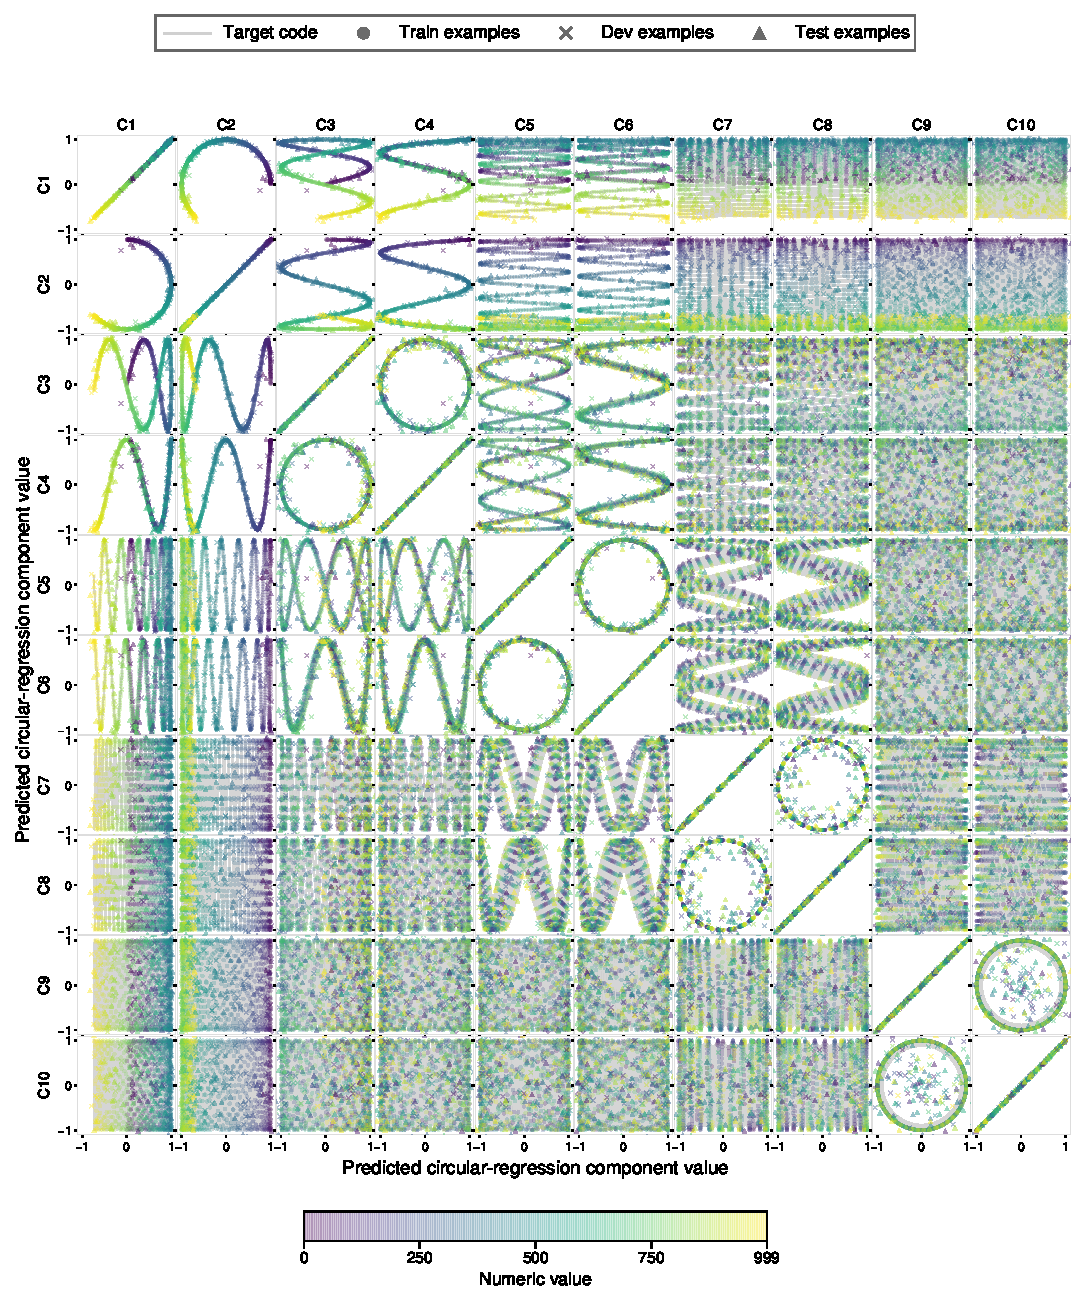
\includegraphics[width=.70\textwidth]{../figures/fig_circular_component_pairs.pdf}
\caption{Low decoding error coexists with large errors in high-frequency components.
Gray curves show the fixed code for 0--999; points are circular-regression predictions for 800 training, 100 development, and 100 test values (Figure~\ref{fig:decodability}).
Departures from the gray curves reveal code errors that accurate numerical decoding can conceal.
Axes are clipped to $[-1.1,1.1]$; statistics use unclipped predictions.}
\label{fig:circular-components}
\end{figure*}

\paragraph{Prompt variants and parsed outputs.}
\label{app:prompt-style-examples}

Table~\ref{tab:prompt-style-examples} illustrates the five prompt variants and their output format with cached Llama-3.2-1B development cases from the complexity sweep.
These examples include incorrect answers alongside exact matches, but all displayed continuations parse as numbers.
The Llama-3.1-8B condition in Figure~\ref{fig:decodability}c is evaluated separately.

\begin{table*}[t]
\centering
\small
\setlength{\tabcolsep}{3pt}
\renewcommand{\arraystretch}{1.08}
\begin{tabularx}{\textwidth}{@{}>{\raggedright\arraybackslash}p{0.08\textwidth}>{\raggedright\arraybackslash}p{0.09\textwidth}>{\raggedright\arraybackslash}p{0.09\textwidth}>{\raggedright\arraybackslash}X>{\raggedright\arraybackslash}p{0.09\textwidth}@{}}
\toprule
Case & Source value & Expected output & Prompt shown to model & Output \\
\midrule
\multicolumn{5}{@{}l}{\textbf{Addition Formula}: $s + x = y$; $x + s = y$}\\
correct & $s=87$ & $y=95$ & 279+3=282; 92+851=943; 599+283=882; 8+87= & 95 \\
wrong & $s=455$ & $y=514$ & 590+48=638; 402+339=741; 43+931=974; 59+455= & 614 \\
\addlinespace[0.25em]
\multicolumn{5}{@{}l}{\textbf{Addition Verbalized}: The result of $s$ plus $x$ is $y$; The result of $x$ plus $s$ is $y$}\\
correct & $s=87$ & $y=95$ & The result of 8 plus 87 is  & 95 \\
wrong & $s=183$ & $y=219$ & The result of 183 plus 36 is  & 19 \\
\addlinespace[0.25em]
\multicolumn{5}{@{}l}{\textbf{Subtraction Formula}: $s - x = y$; $x - s = y$}\\
correct & $s=87$ & $y=74$ & 279-189=90; 848-738=110; 54-29=25; 87-13= & 74 \\
wrong & $s=274$ & $y=12$ & 788-710=78; 133-24=109; 917-916=1; 286-274= & 112 \\
\addlinespace[0.25em]
\multicolumn{5}{@{}l}{\textbf{Subtraction Verbalized}: The result of $s$ minus $x$ is $y$; The result of $x$ minus $s$ is $y$}\\
correct & $s=87$ & $y=65$ & The result of 152 minus 87 is  & 65 \\
wrong & $s=194$ & $y=193$ & The result of 194 minus 1 is  & 3 \\
\addlinespace[0.25em]
\multicolumn{5}{@{}l}{\textbf{Copying}: $s = y$}\\
correct & $s=121$ & $y=121$ & 643 = 643; 2 = 2; 431 = 431; 121 =  & 121 \\
\bottomrule
\end{tabularx}
\caption{The five prompt variants place the source value $s$ in different arithmetic and textual contexts; $y$ is the expected output.
Examples are Llama-3.2-1B development cases from the complexity sweep.
The displayed continuations parse directly as the numbers used for evaluation.}
\label{tab:prompt-style-examples}
\end{table*}



\paragraph{Probe complexity.}
\label{sec:probe-capacity}

The complexity analysis measures how held-out value-decoding error at the probed token position changes within each probe method.
For PLS and circular probes, the horizontal axis gives the retained component count or sinusoidal code dimension.
For ridge probes, effective degrees of freedom equal $\sum_j s_j^2/(s_j^2+\lambda)$, where $s_j$ are the singular values of the centered training activation matrix and $\lambda$ is the ridge penalty.
Figure~\ref{fig:probe-capacity-paths} reports all relative layers in a six-model sweep on the fixed value-disjoint partition, averaged over five prompt variants.
The models are Llama 3.2 (1B and 3B), Llama 3.1 (8B), OLMo 3 (7B), OLMo 2 (13B), and GPT-OSS 20B.
The eleven relative layers run from 0 to 1 in steps of .1, corresponding to the embedding output through the final Transformer block.

\begin{figure*}[t]
    \centering
    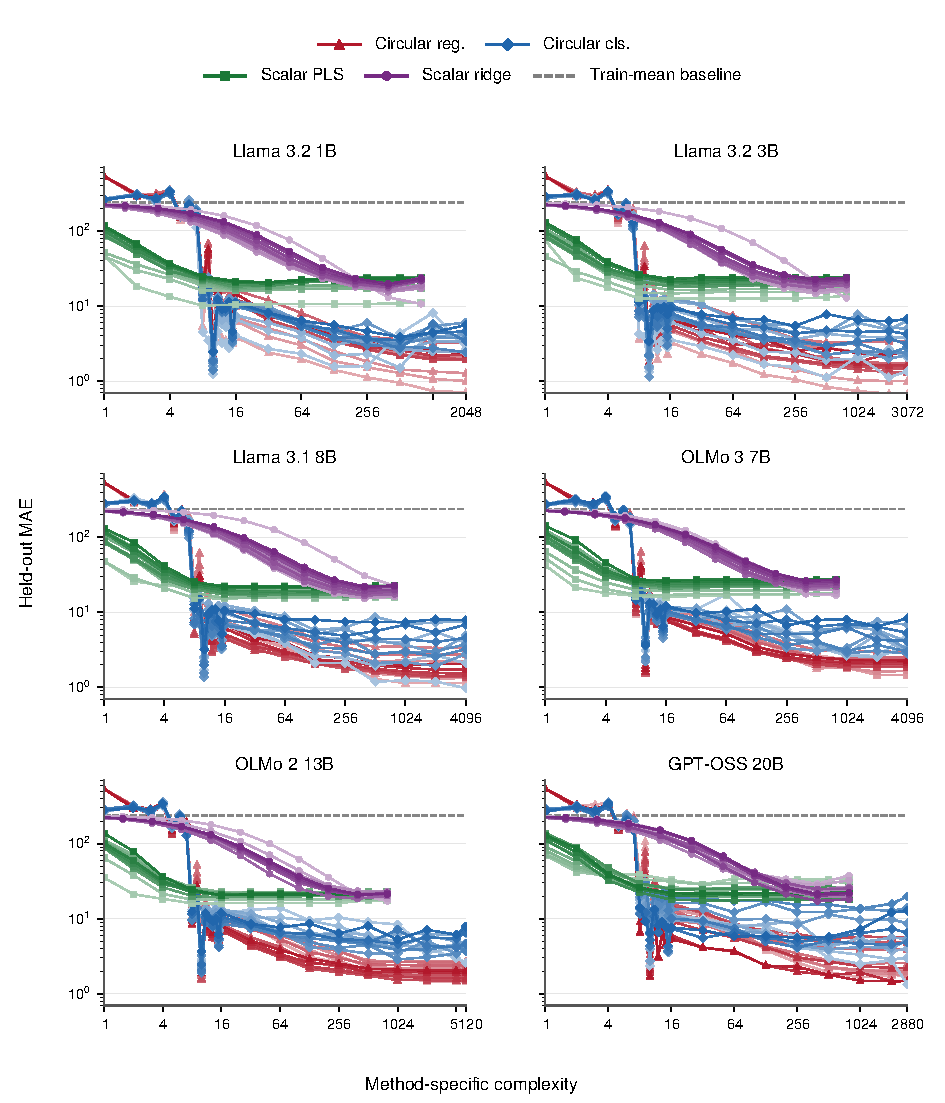
\includegraphics[width=\textwidth]{../figures/fig_probe_capacity_paths.pdf}
    \caption{Decoding error varies with method-specific tuning quantities.
    Curves show held-out MAE at the probed token position for six models and all relative layers, averaged over five prompt variants on one fixed value-disjoint partition; lower is better.
    Color denotes probe method, lighter traces denote shallower layers, and the dashed gray line marks the training-mean baseline.
    The horizontal axis gives ridge effective degrees of freedom, PLS component count, or circular-code dimension, with model-specific ranges.
    These sweeps show how decoding responds to complexity within each probe method; comparing efficiency across methods additionally requires a common cost measure.}
    \label{fig:probe-capacity-paths}
\end{figure*}

Figure~\ref{fig:decodability}d uses separate fits on the centroids and split of panel (c); the classifier with code dimension 10 has MAE 1.09, versus 1.14 in (c).

The tuning optima vary across probe methods and models in the six-model sweep.
Ridge probes have a median optimum of about 400 effective degrees of freedom; PLS probes typically reach minimum MAE with 16 components.
Circular classification reaches a median best MAE of 2.45 with a ten-dimensional code, and circular regression reaches a median best MAE of 1.74 at a median code dimension of 1024.
Code dimension, however, measures only part of classification complexity: Figure~\ref{fig:decodability}d keeps the learned projection width fixed at 100.


\paragraph{Transfer across prompt variants.}

Prompt-variant transfer tests the invariance of fitted linear maps in Section~\ref{sec:weak-strong}.
Figure~\ref{fig:prompt-family-pls-transfer} reports PLS transfer across six models, five prompt variants, and eleven relative layers.
This transfer panel uses Llama 3 8B; the other five models match the complexity sweep.
Each integer is represented by an equal-weight mean over all available contexts within its variant.
To assess whether mean alignment reduces transfer error, the mean-alignment control estimates each variant mean from the 800 training values, translates source and target activations to the equal-variant global mean, and keeps the source direction and gain fixed.
As a complementary invariance test, the direction panel compares unit directions from independently trained PLS probes by cosine similarity, displaying each cross-variant pair once.
These comparisons use the same value-disjoint partition of 800 training, 100 development, and 100 test integers.

\begin{figure*}[t]
\centering
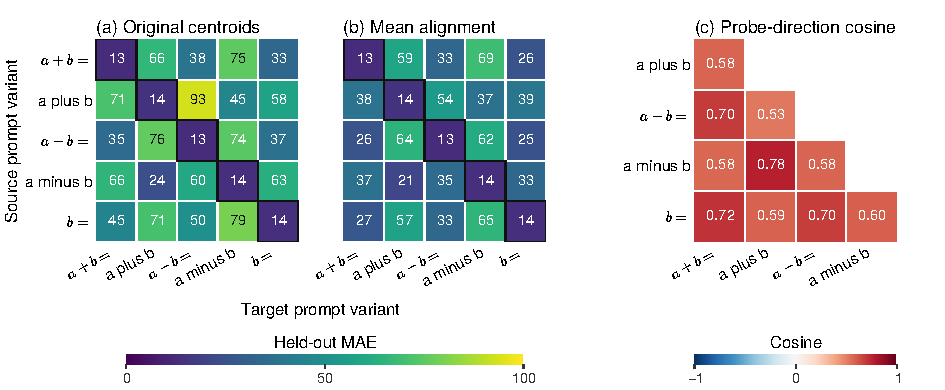
\includegraphics[width=\textwidth]{../figures/fig_prompt_family_pls_transfer.pdf}
\caption{Aligning prompt-variant means reduces transfer error, with a large gap from within-variant decoding.
Panels (a) and (b) show held-out MAE before and after mean alignment; panel (c) shows cosine similarity between independently fitted PLS directions.
Cells average six models and eleven relative layers on one 800/100/100 value-disjoint split.
Mean alignment uses target-variant training activations and freezes the source direction and gain.
Outlines mark probes evaluated in their training variant, providing a reference for the larger transfer errors in the other cells, including after mean alignment.}
\label{fig:prompt-family-pls-transfer}
\end{figure*}

\paragraph{Context averaging.}

Figures~\ref{fig:prompt-style-transfer}--\ref{fig:prompt-transfer-ridge} report context averaging for circular regression, scalar PLS, and scalar ridge on the same six-model, eleven-layer panel.
For each integer and prompt variant, we compare one deterministic context with the mean activation over all available contexts.
To compare these aggregation conditions at fixed complexity, we choose the tuning quantity once from single-context within-variant development performance and hold it fixed; both conditions share a value-disjoint partition of 800 training, 100 development, and 100 test integers.
With these choices fixed, context averaging reduces mean within-variant held-out MAE from 14.1 to 9.6, but cross-variant mean MAE increases from 49.9 to 50.6, leaving the transfer gap intact.

\begin{figure*}[t]
\centering
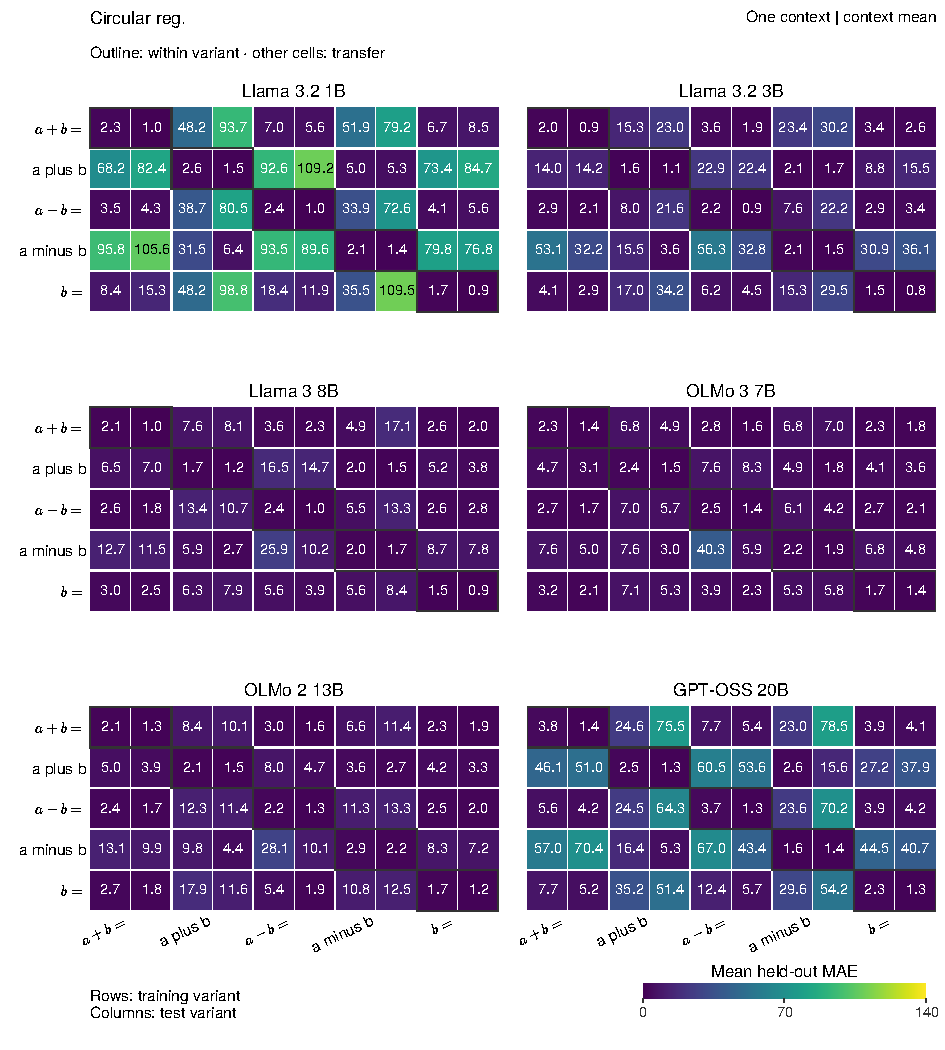
\includegraphics[width=\textwidth]{../figures/fig_prompt_variant_transfer_circular_reg.pdf}
\caption{Circular regression decodes values accurately within prompt variants, with larger transfer errors.
Each panel shows one model; rows give training variants and columns give test variants.
Each cell compares one context per value (left) with the mean over contexts (right).
The code dimension is selected on single-context within-variant development data and fixed between conditions.
Cells report held-out MAE averaged over eleven relative layers; diagonal cells show within-variant decoding.
Lower is better; colors use a shared scale capped at 140, and values are rounded to one decimal.}
\label{fig:prompt-style-transfer}
\end{figure*}

\begin{figure*}[t]
\centering
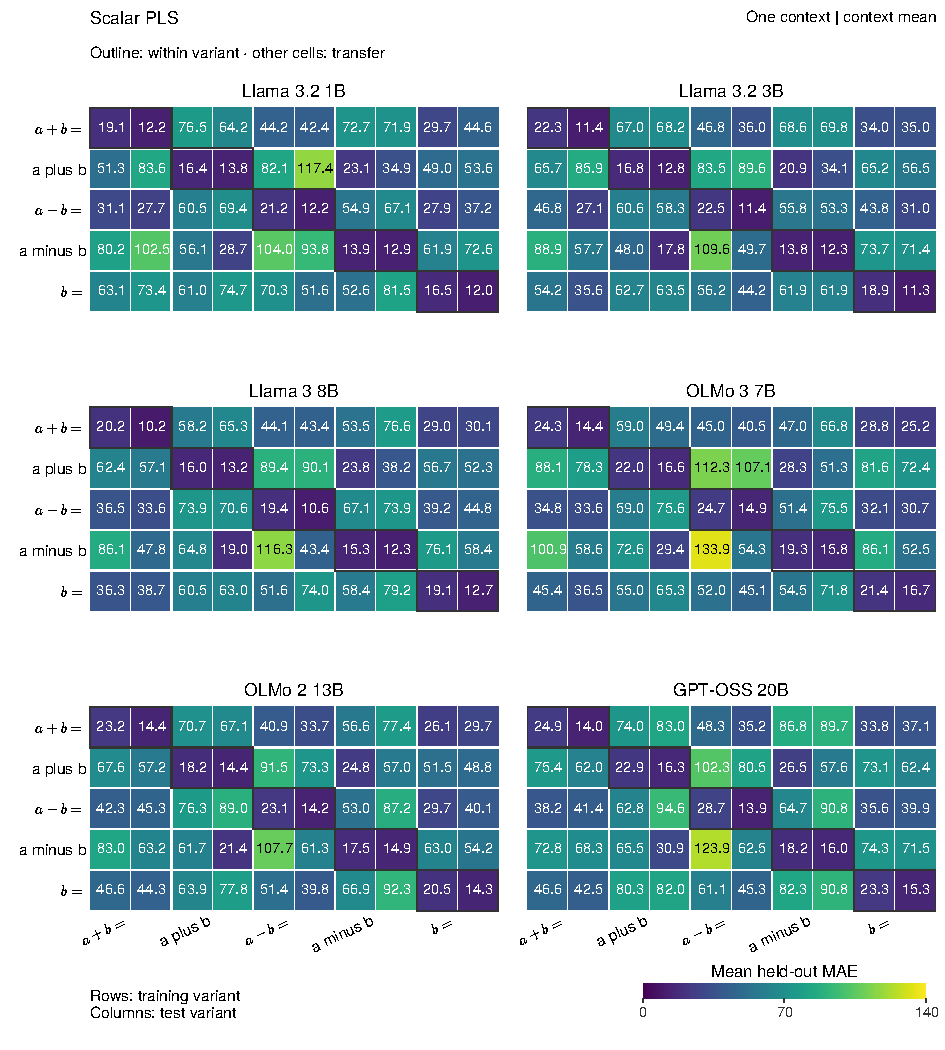
\includegraphics[width=\textwidth]{../figures/fig_prompt_variant_transfer_scalar_pls.pdf}
\caption{Scalar PLS probes show a persistent transfer gap after context averaging.
Rows give training variants and columns give test variants; each cell compares one context per value (left) with the mean over contexts (right).
The PLS component count is selected on single-context within-variant development data and fixed between conditions.
Cells report held-out MAE averaged over eleven relative layers; colors use a shared scale capped at 140.
Values are rounded to one decimal; the remaining conditions match Figure~\ref{fig:prompt-style-transfer}.}
\label{fig:prompt-transfer-pls}
\end{figure*}

\begin{figure*}[t]
\centering
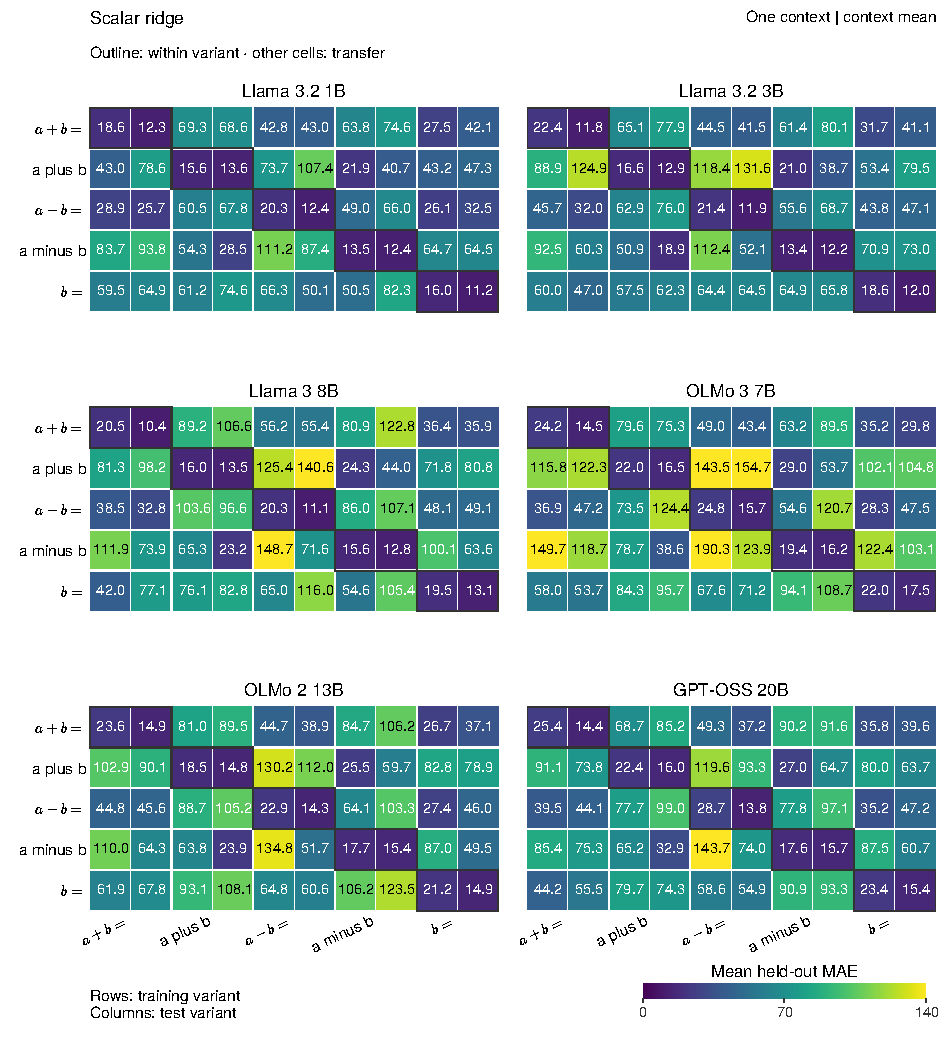
\includegraphics[width=\textwidth]{../figures/fig_prompt_variant_transfer_scalar_ridge.pdf}
\caption{Context averaging lowers within-variant scalar ridge error, with mixed effects on transfer.
Rows give training variants and columns give test variants; each cell compares one context per value (left) with the mean over contexts (right).
The ridge penalty is selected on single-context within-variant development data and fixed between conditions.
Cells report held-out MAE averaged over eleven relative layers; colors use a shared scale capped at 140.
Values are rounded to one decimal; the remaining conditions match Figure~\ref{fig:prompt-style-transfer}.}
\label{fig:prompt-transfer-ridge}
\end{figure*}

\paragraph{Steering design and accuracy.}

Figure~\ref{fig:numerical-sufficiency-atlas}a--c uses the same scalar ridge and circular-regression fits for numerical decoding and steering at the Llama-3.1-8B layer-10 source-number token.
Both probes are fitted to individual prompts for the 800 training values, using the partition and prediction rules above.
Decoding and steering share 100 development prompts, held out from fitting and reused from the earlier steering evaluation.
Decoding MAE is 19.1 for scalar ridge and 1.78 for circular regression.
The matched activations use checkpoint revision \texttt{d04e592b}, FP16, and eager attention.
For an addition-formula prompt \texttt{$x$+$s$=}, replacing source operand $s$ with target operand $t$ gives the counterfactual answer $x+t$.
We evaluate 20 target replacements per prompt, giving 2,000 interventions shared by all displayed methods.
Each source prompt has three demonstrations, an auxiliary operand, and a source operand at the edited token position.
Demonstration prefixes vary across prompts; 51 prompts edit the left operand and 49 edit the right operand.
These targets span ten displacement ranges between 1 and 500.
We assess success by exact accuracy, counting top-1 continuations equal to $x+t$, and lenient accuracy, permitting an absolute difference of at most 10, inclusive.
Under both criteria, nonnumeric continuations count as failures.

Centroid shifts add the difference between target and source value centroids, each averaged over the 20 auxiliary operands specified above.
The displayed edit projects this difference into a 64-dimensional PCA subspace fitted on all 1,000 value centroids, including development and test values; its use of target activations makes it a target-informed control.
The PCA shift reaches 99.75\% exact accuracy, the full centroid shift 99.90\%, and replacement with the matched counterfactual activation 99.95\%.

For uncertainty in steering accuracy, Figure~\ref{fig:numerical-sufficiency-atlas}c gives 95\% percentile intervals from 10,000 paired resamples of the 100 source prompts (seed 1729), retaining all twenty targets for each sampled source.
Because the probes and target set are fixed, these intervals measure variation across source prompts.
For zero exact successes, resampling cannot estimate an upper bound on future success, so the figure reports observed counts without an interval.

\paragraph{Probe-derived edits.}
\label{sec:numerical-probe-geometry}

For circular regression, let row activation $h\in\mathbb{R}^{1\times d}$ map to the fixed sinusoidal Fourier code $\phi(v)\in\mathbb{R}^{1\times 10}$ through
\begin{equation}
 z(h)=hW+b,\qquad W\in\mathbb{R}^{d\times 10}.
\end{equation}
The probe-derived edit for source value $s$ and target value $t$ is
\begin{equation}
 \Delta h=\bigl[\phi(t)-\phi(s)\bigr]W^{+},
\end{equation}
where $W^{+}$ is the Moore--Penrose pseudoinverse.
When $W$ has full column rank, this is the minimum-norm activation edit producing the requested code difference.
Because the construction uses the label code $\phi(s)$, any discrepancy between the predicted source code $z(h_s)$ and $\phi(s)$ persists after editing.
The predicted code also leaves null-space components undetermined: adding such a component preserves the prediction but can affect downstream computation.
Scalar ridge and scalar PLS probes use this construction with a one-dimensional output.

\FloatBarrier

\appendixsection{Control and Number-Property Experiments}
\label{sec:numerical-control-dimension}

This appendix documents property decoding and deletion, coefficient-based control, and selective parity edits in the main text.
The Llama-3.1-8B addition experiments use the activation extraction and 800/100/100 value-disjoint partitions specified in Appendix~\ref{sec:numerical-probe-setup}.
Appendix~\ref{sec:reproducibility} describes the archived observations and configurations.

\paragraph{Property decoding and deletion.}
\label{sec:number-property-geometry}

The decoding analysis fits ridge classifiers to the nineteen categorical properties in Figure~\ref{fig:number-property-accessibility-main}a, selecting $\lambda\in\{.01,.1,1,10,100,1000\}$ by development balanced accuracy.
We evaluate ten value-disjoint splits and retain those whose test partition contains every training class: six for digit count, eight for distinct-digit count, and all ten for the other properties.
The figure reports means and ranges over these retained splits.

For deletion (Figure~\ref{fig:causal-use}c), each split has a rank-41 basis fitted on addition-formula activations to magnitude and the nineteen categorical properties using the procedure below.
We remove the activation component in this basis at the source-number token and compare with rank-matched bases fitted to shuffled labels.
Evaluation covers seven tasks, with 1,000 prompts per task and 639 distinct source values overall.
Because the ten splits overlap in their evaluation values, the 95\% percentile intervals use 2,000 resamples clustered by source value, averaging control seeds within each split, task, and value before resampling and weighting prompts equally.
Holding the fitted bases fixed restricts these intervals to evaluation-sample uncertainty.

\paragraph{Coefficient prediction and search.}
\label{sec:property-coefficient-control}

To construct a basis in which several properties can share a direction, we encode magnitude and one-hot categorical labels in a 68-column target matrix, centering and normalizing each property's block using training values.
The resulting centered matrix has rank 41, which sets the maximum basis rank.
To estimate its directions, we repeatedly fit one rank-one probe per property on a deterministic inner 80\% of the 800 training values.
We select the candidate that best predicts its property's target block from residual activations on the inner 20\%, refit it on all 800 values, and project out its direction before the next step.
Each direction is labeled by its selecting property, although other properties can also load on it.

The coefficient comparison and search below use the full rank-41 basis.
Within this basis, Figure~\ref{fig:numerical-sufficiency-atlas}f compares coefficient prediction on 400 interventions from 20 held-out source prompts, with 20 target replacements per prompt.
The independent method sums edits predicted separately from source and target labels for each property.
For categorical properties, labels predict the assigned coefficients and their target-minus-source differences define the edit; for magnitude, the edit uses the inverse of a calibrated prediction along the first PLS direction.
Joint ridge and radial basis function (RBF) kernel ridge additionally use the source activation projected into the basis, together with both label sets, to predict coefficients of counterfactual patch displacements in that basis.
To fit and select these joint predictors, the 100 source prompts are partitioned into 60 training, 20 validation, and 20 test prompts (seed 20260729).
After selecting hyperparameters to minimize validation coefficient error, we refit the models on the 80 training and validation prompts.
Target values occur in both training and evaluation partitions, and intervention doses differ among methods.
The independent sum yields 0/400 exact outputs, compared with 77\% for joint ridge and 80\% for RBF ridge.
The nonzero rates have 95\% percentile intervals from 10,000 bootstrap resamples of the 20 source prompts (seed 20260826).
Under these comparison conditions, most of the observed improvement occurs when coefficients are predicted jointly with source activations available.

A separate experiment tests what edits selected using the requested output can achieve within the same rank-41 basis.
It evaluates all 2,000 interventions from the 100 source prompts, with projection into the basis capturing 53\% of the exact-patch displacement energy.
Selecting coefficients by the requested target token's probability under the exact-patch norm budget nevertheless reaches 99.5\% exact accuracy.

\paragraph{Selective parity interventions.}
\label{sec:property-reasoning}

The Llama classification test in Figure~\ref{fig:number-property-accessibility-main}b,c uses structured ten-shot question--answer prompts and a parity direction fitted on 800 training numerals.
We add the direction at the query numeral after Transformer block 9 (zero-based index), with dose $\alpha=16$ selected on development values, giving mean edit norm 7.74.
At this dose, the edit preserves the numeral and flips its parity label in 93 of 100 baseline-correct test prompts, compared with 3 for a norm-matched random direction.
This label-flipping result contrasts with parity directions fitted on addition formulas, which achieve perfect in-format decoding but produce zero contradictions when transferred at the same $L_2$ dose.
They instead change the numeral coherently in 50 cases, supporting the context dependence of the intervention effect.

The enumeration test uses a fitted Qwen3.6-27B parity direction (value-disjoint fit, seed 1729).
Zero-shot prompts list ten numbered inputs and request the odd numerals in their original order.
We run the model in bfloat16 and use chat templates with thinking disabled, allowing at most 64 output tokens (protocol seed 20260718).
We edit the targeted numeral's final-digit activation at layer 19.
Dose $\alpha=12$ is selected from $\{2,4,8,12,16\}$ on 30 development lists by maximizing exact counterfactual-set accuracy subject to at least 98\% source fidelity and untargeted membership accuracy.
At the selected dose, the edit inserts the targeted even numeral into an otherwise unchanged list of odd numerals in 48 of 50 baseline-correct test lists.
Norm-matched random, wrong-sign, and delimiter-location controls yield 0, 10, and 3 such contradictions, respectively.
The nonzero wrong-sign and delimiter effects qualify the specificity of the selected direction and activation site.

\FloatBarrier

\appendixsection{Reproducibility and Computational Resources}
\label{sec:reproducibility}

\paragraph{Released artifacts.}

The code and data archives accompany the arXiv version as ancillary files, available from its abstract page.
They contain observations for the quantitative panels in Figures~\ref{fig:lrh-mentions}, \ref{fig:decodability}--\ref{fig:numerical-sufficiency-atlas}, with a map from each panel to its inputs and outputs.
The software archive's \texttt{README.md} and \texttt{EXPERIMENT\_MAP.md} describe these mappings and the reproduction commands; the data archive's \texttt{README.md} describes the distributed observations.
The CPU-only workflow verifies SHA-256 manifests and recomputes metrics, uncertainty intervals, and numerical plots, including the six-model complexity sweep and supporting appendix analyses, without downloading a model.
For model-forward reproduction, the archives also include experiment sources and configurations with synthetic prompts and fixed intervention inputs; running these sources uses public checkpoints and regenerates activation caches.
The archives exclude model weights, activation caches, and published-paper PDFs.

The numerical data consist of generated integers, arithmetic prompts, and number-property questions, with corresponding model outputs and derived statistics.
The prompts use English and Arabic numerals and contain no personally identifying or offensive text.
The data contain no personal records or demographic attributes.

\paragraph{Models and software.}

Table~\ref{tab:experimental-models} identifies the model families used in the numerical experiments and links their model cards or license terms.
The archives record public checkpoint identifiers and available revisions.

\begin{table}[H]
\centering
\small
\setlength{\tabcolsep}{3pt}
\renewcommand{\arraystretch}{1.08}
\begin{tabularx}{\linewidth}{@{}>{\raggedright\arraybackslash}p{.42\linewidth}>{\raggedright\arraybackslash}p{.18\linewidth}>{\raggedright\arraybackslash}X@{}}
\toprule
Model family & Parameters & Model license \\
\midrule
\href{https://huggingface.co/meta-llama/Llama-3.2-1B}{Llama 3.2} & 1B, 3B & Llama 3.2 Community \\
Llama 3/3.1 \citep{grattafiori2024llama} & 8B & \href{https://huggingface.co/meta-llama/Meta-Llama-3-8B}{Llama 3}/\href{https://huggingface.co/meta-llama/Llama-3.1-8B}{3.1 Community} \\
OLMo 2 \citep{teamolmo2025olmo2} & 13B & \href{https://huggingface.co/allenai/OLMo-2-1124-13B}{Apache 2.0} \\
OLMo 3 \citep{teamolmo2026olmo3} & 7B & \href{https://huggingface.co/allenai/Olmo-3-1025-7B}{Apache 2.0} \\
GPT-OSS \citep{openai2025gptoss} & 21B total; 3.6B active & \href{https://huggingface.co/openai/gpt-oss-20b}{Apache 2.0} \\
Qwen3.6 \citep{qwen2026qwen36} & 27B & \href{https://huggingface.co/Qwen/Qwen3.6-27B}{Apache 2.0} \\
\bottomrule
\end{tabularx}
\caption{Model sizes and licenses for the numerical experiments.
Parameter counts are rounded; GPT-OSS uses a mixture of experts.}
\label{tab:experimental-models}
\end{table}

Model execution and intervention hooks use PyTorch \citep{paszke2019pytorch} and Transformers \citep{wolf2020transformers}.
Array operations use NumPy \citep{harris2020numpy}; probe fitting uses scikit-learn \citep{pedregosa2011scikit}.
The CPU verification environment pins NumPy 2.3.3, \href{https://pandas.pydata.org/}{pandas} 3.0.2, and \href{https://matplotlib.org/}{Matplotlib} 3.10.8.
The archives include locked environments for selected model-forward workflows.
Appendices~\ref{sec:numerical-probe-setup} and~\ref{sec:numerical-control-dimension}, together with the archived configurations, specify model execution, preprocessing, and evaluation settings.

\paragraph{Artifact licenses.}

Our analysis code uses the MIT license; our original derived measurements and annotations use CC BY 4.0.
Each archive includes a license file.
Third-party libraries and model weights are obtained separately from their original distributors under the applicable terms, including the model licenses in Table~\ref{tab:experimental-models}.

\paragraph{Computational resources.}

GPU runs used NVIDIA H200 accelerators on ABCI and an NVIDIA GB10 workstation.
We estimate approximately 20 accelerator-hours and 100 CPU core-hours for the reported analyses and development runs from partial job records.
These records account for 10 NVIDIA H200 allocation-hours, 1.1 NVIDIA GB10 hours, and approximately 78 CPU core-hours, counting multi-GPU allocation-hours as elapsed wall time multiplied by the number of allocated devices.
We extend the recorded totals upward to cover shared cache construction, aggregation, and runs with incomplete timing records, excluding the compute used to pretrain the public checkpoints.
Reusing released checkpoints and cached activations reduces additional computation and its associated environmental cost.

\paragraph{Research considerations.}

The review discusses refusal suppression \citep{arditi2024refusal}, which can bypass model safeguards.
The framework's claim distinctions and the Limitations section address the risk of inferring model computation from decoding or intervention results alone.

\paragraph{AI assistance.}

We used OpenAI Codex for literature search and evidence coding, preparing and checking experiment and visualization code, and manuscript revision.
Appendices~\ref{sec:lrh-search} and~\ref{sec:evidence-comparison} document the literature classification and rating procedures.
The authors reviewed the manuscript and analyses and take responsibility for the reported claims and results.

\clearpage
\appendixsection{Geometric Illustrations of Decoding and Intervention}
\label{sec:geometric-illustrations}

This appendix specifies the local approximation and probe-output display in Figure~\ref{fig:decodability} and the schematic interventions in Figure~\ref{fig:numerical-sufficiency-atlas}.
We use row activation vectors, as in Appendix~\ref{sec:numerical-probe-geometry}.
The intervention constructions show how accurate decoding and valid individual edits can coexist with unsuccessful behavioral control.
We then derive the retained null-space component and use a curved-path example to explain why probe predictions do not determine behavior away from the original activations.

\paragraph{Local linearization.}
For a twice continuously differentiable decoder $f:\R^d\to\R$, the linear approximation at $h_0$ is
\begin{equation}
a(h)=f(h_0)+(h-h_0)\nabla f(h_0).
\end{equation}
If the Hessian operator norm is bounded by $L$ within radius $r$, Taylor's theorem gives $|f(h)-a(h)|\leq Lr^2/2$ throughout that region.
An evaluation restricted to this region can admit accurate linear prediction even when $f$ is nonlinear elsewhere (Figure~\ref{fig:decodability}a).

\paragraph{Probe outputs in Figure~\ref{fig:decodability}b.}
The display combines the scalar ridge prediction $\hat v_{\rm ridge}$ with predicted cosine and sine components $\hat c,\hat s$ as $((\hat v_{\rm ridge}-499.5)/499.5,\hat c,\hat s)$.
The selected sine--cosine pair has angular frequency $1000^{-6/10}$ (period approximately 396).
We display all 1,000 values, including 800 fitting values, with an orthographic camera and uniform zoom to preserve linear scales; the gray helix provides the target-code reference.

\paragraph{Circular-code matching in Figure~\ref{fig:numerical-sufficiency-atlas}d.}
The illustrated helix segment is
\begin{equation}
h(t)=(\cos(\pi t/2),\sin(\pi t/2),t),\quad 0\leq t\leq1.
\end{equation}
The linear projection $P(x,y,z)=(x,y)$ yields a circular code, decoded as $d(x,y,z)=2\operatorname{atan2}(y,x)/\pi$; downstream computation uses $F(x,y,z)=z$.
The decoded value and downstream output both equal $t$ on the original segment.
Editing the circular components from source $h(0)=(1,0,0)$ to those of target $h(1)=(0,1,1)$ gives $h'=(0,1,0)$.
The edit matches the target code and predicts $d(h')=1$, but retains the source output $F(h')=0$.

\paragraph{Combining property edits in Figure~\ref{fig:numerical-sufficiency-atlas}e.}
The surface is $h(u,v)=(u,v,uv)$ for $0\leq u,v\leq1$, with property probes $P(x,y,z)=(x,y)$ and downstream output $F(x,y,z)=z$.
From source $h(0,0)=(0,0,0)$, the individual displacements $(1,0,0)$ and $(0,1,0)$ reach valid surface activations with the respective property set to 1.
Their sum yields $(1,1,0)$: both properties match the joint target $h(1,1)=(1,1,1)$, but the output is still 0 instead of 1.
Reaching the joint target requires the interaction term in the third component.

\paragraph{Projection and the minimum-norm edit.}
The null-space issue in Section~\ref{sec:sufficiency} applies to any linear projection, including one that approximately preserves distances between sampled activations \citep{johnson1984extensions}.
Let $P\in\R^{d\times k}$ with $k<d$, pseudoinverse $P^+$, and projector $Q=PP^+$ onto its column space.
The minimum-norm edit matching the target projection gives
\begin{equation}
\begin{split}
h'&=h_s+(h_tP-h_sP)P^+\\
  &=h_tQ+h_s(I-Q).
\end{split}
\label{eq:projection-edit}
\end{equation}
It retains the source component in the probe's null space, with $h'-h_t=(h_s-h_t)(I-Q)$.
The distance guarantee applies to the original sample; an edited state outside it can share the target's projection.
Matching the projection guarantees equal behavior when $F(h)=G(hP)$ on the original and edited states.
Dependencies on the retained component can change the outcome.
The same identity holds for a linear probe $hA+b$, since the bias cancels in target-minus-source differences.

\paragraph{Chord interventions on a curved manifold.}
The curved paths discussed in Section~\ref{sec:sufficiency} motivate a second example of this ambiguity.
In the parabola construction adapted from \citet{wurgaft2026manifold}, $h(t)=(t,t^2)$ and the probe $d(x,y)=x$ decodes $t$ exactly.
The chord between $h(-a)$ and $h(a)$ is $\widetilde h(t)=(t,a^2)$ for $a>0$ and $t\in[-a,a]$.
Its interior lies off the parabola but has the same probe predictions.
To compare behaviors consistent with the original activations, consider downstream computations
\begin{equation}
F_\lambda(x,y)=x+\lambda(y-x^2).
\end{equation}
All output $t$ on the parabola but $t+\lambda(a^2-t^2)$ on the chord, so varying $\lambda$ changes intervention behavior despite agreement on every original activation.

\end{document}
